\documentclass[a4paper,10pt]{article}

%Les packages pour écrire des math
\usepackage{amsmath}
\usepackage{amsthm}
\usepackage{amssymb}
\usepackage{mathabx}
\usepackage{dsfont} %Fonction caractéristique
\usepackage{stmaryrd}


\usepackage{listings}
\usepackage[authoryear]{natbib}


\usepackage{hyperref}
\usepackage{url}

\usepackage{algorithm}
\usepackage{algorithmic}

\usepackage[francais]{babel}	
\usepackage[utf8]{inputenc}

\usepackage{graphicx}
%\usepackage{pst-solides3d}
\graphicspath{ {./images/} }
\usepackage[font=small,labelfont=bf]{caption}


\textwidth17cm
\oddsidemargin-0.38cm
\textheight23cm
\topmargin-2cm
\pagestyle{plain}


\renewcommand {\algorithmicrequire } {\textbf{\textsc{Entrée(s):} } }
\renewcommand {\algorithmicensure } {\textbf{\textsc{Sortie:} } }
\renewcommand {\algorithmicwhile } {\textbf{Tant que} }
\renewcommand {\algorithmicdo } {\textbf{faire} }
\renewcommand {\algorithmicendwhile } {\textbf{fin du Tant que} }
\renewcommand {\algorithmicif } {\textbf{Si} }
\renewcommand {\algorithmicfor } {\textbf{Pour} }
\renewcommand {\algorithmicendfor } {\textbf{fin du Pour} }
\renewcommand {\algorithmicthen } {\textbf{alors} }
\renewcommand {\algorithmicendif } {\textbf{fin du Si} }
\renewcommand {\algorithmicelse } {\textbf{Sinon} }
\renewcommand {\algorithmicreturn } {\textbf{Renvoyer} }

\newtheorem{theorem}{Théorème}[section]
\newtheorem{conjecture}{Conjecture}
\newtheorem{lemma}{Lemme}
\newtheorem{proposition}{Proposition}
\newtheorem{corollary}{Corollaire}
\newtheorem{definition}{Définition}
\newtheorem{example}{Exemple}
\newtheorem{note}{Note}



\begin{document}
	
	\hypersetup{pdfborder=0 0 0}
	\newcommand{\HRule}{\rule{\linewidth}{0.5mm}}
	\begin{center}
		\textsc{\LARGE Laboratoire des Sciences du Climat} \\[0.3cm]
		\textsc{\LARGE et de l'Environnement}\\[1.5cm] 
		\HRule \\[0.5cm]
		{ \huge \bfseries Upscaling et Downscaling dans la modélisation hydrologique  }\\[0.4cm] 
		\HRule \\[1.5cm]
	\end{center}
	
	\begin{minipage}{0.4\textwidth}
		\begin{flushleft} \Large
			\emph{Auteur}\\
		\end{flushleft}
	\end{minipage}
	~
	\begin{minipage}{0.4\textwidth}
		\begin{flushright} \Large
			\emph{Maîtres de stage} \\
		\end{flushright}
	\end{minipage}\\[0.5 cm]
	\begin{minipage}{0.4\textwidth}
		\begin{flushleft} \large
			\textsc{Mathis Deronzier}\\
			\textsc{Mines Saint-Étienne}
		\end{flushleft}
	\end{minipage}
	~
	\begin{minipage}{0.4\textwidth}
		\begin{flushright} \large
			\textsc{Emmanuel Mouche}\\
			\textsc{C.E.A.}\\
			\textsc{Mathieu Vrac}\\
			\textsc{C.E.A.}
		\end{flushright}
	\end{minipage}\\[2cm]
	\begin{center}
		\textsc{\Large Stage de recherche de master 2}\\[0.5cm]  
		\large Avril-Septembre\\2021\\[2cm]
	\end{center}
	
	\newpage
	\tableofcontents
	\newpage
	
	\section{Downscaling}
	\label{dwnsc}
	Le downscaling (voir par exemple \cite{vrac2012dynamical} et \cite{ayar2016intercomparison}) est une méthode statistique utilisée dans les sciences du climat permettant d'améliorer les modèles de prédiction. À partir des données obtenues par un modèle de simulation (modèle de circulation général, modèle climatique régional) et des données réelles on cherche à corriger les biais systématiques. Le nom ``downscaling'' vient du fait que l'on cherche souvent à faire des prédictions sur un point particulier du domaine prédit par le modèle de prédiction. Cette méthode est très utile dans la pratique où l'on a des simulateurs donnant des informations sur des maillage de grande distance de grille ($\sim 200km$). Dans notre cas, nous utilisons le downscaling pour prédire les variables climatiques de \textit{précipitation} et d'\textit{évapotranspiration} sur le bassin du \textbf{Little Washita} ($\sim 30\times30 km^2$). Nous avons testé nos méthodes à partir de deux jeux de données: les données NARRs (voir section \ref{NARRs}) ainsi que celles de l'IPSL.
	
	Pour formuler rigoureusement l'approche du downscaling nous introduisons des hypothèses communément admises dans les sciences du climat. On suppose que les variables étudiées sont des variables aléatoires dépendantes du temps et de l'espace. On appelle $\mathcal{M}(\Omega,\mathbb{R})$ l'espace des variables aléatoires réelles et $S(\mathbb{R})$ la spère unité dans $\mathbb{R}^3$, on suppose de plus que l'on peut faire correspondre chaque point de la terre à un point de la sphère unité.
	
	\begin{definition}
		\label{terre}
		Pour une variable quantitative $V$ à valeur dans $\mathbb{R}$, on appelle $\mathcal{T}_V$ la fonction donnant les  valeurs réelle de cette variable sur la terre à un moment donné, formellement (en considérant la terre comme une sphère $\mathcal{S}(\mathbb{R}^3)$) nous avons
		\begin{equation}
			\begin{array}{ccc}
				\mathcal{T}_V: \mathbb{R}_{+}\times\mathcal{S}(\mathbb{R}^{3}) & \to & \mathcal{M}(\Omega,\mathbb{R}).
			\end{array}
		\end{equation}
		Alors, $\mathcal{T}_V(t,x)$ est la valeur de la variable au temps $t$ au point de coordonnée $x$ sur terre.	
	\end{definition}
	
	\begin{definition}
		\label{simu_terre}
		On appelle simulateur de variable quantitative $V$ à valeur dans $\mathbb{R}$, une fonction $S_V$ satisfaisant:
		\begin{equation}
			\begin{array}{ccc}
				S_V: \mathbb{R}_{+}\times\mathcal{S}(\mathbb{R}^{3}) & \to & \mathcal{M}(\Omega,\mathbb{R}).
			\end{array}
		\end{equation}
	\end{definition}
	
	On peut alors estimer la qualité des simulations en mesurant une distance entre la réalisation $\mathcal{T}_V([0,T])$ et celle de $S_V([0,T])$. Le travail du downscaling est de minimiser ces distances. Les géostatistiques essaie de munir ces fonctions de structures particulières pour améliorer les résultats des prédictions (voir par exemple \cite{lindgren2011explicit}).  
	
	\subsection{Introduction à la problématique du downscaling}
	\label{intro-dwnsc}
	Le downscaling consiste à effectuer des transformations sur des variables aléatoire réelles. Pour étudier ces variables aléatoires on introduit ici les notions de \textbf{fonction de répartition} et de \textbf{fonction de répartition empirique} ainsi que celle de \textbf{fonction de densité}. Ces notions sont centrales dans les méthodes de downscaling que nous allons expliquer.
	
	\begin{definition}
		Soit $X$ une variable aléatoire réelle, on appelle \textbf{fonction de répartition de $X$}, $\mathcal{F}_{X}: \mathbb{R}\to [0,1]$ la fonction vérifiant
		\begin{equation}
			\mathcal{F}_{X}(x)=P(X\leq x).
		\end{equation}
	\end{definition}
	
	\begin{definition}
		Soient $X_1,X_2,...,X_n$, n réalisations indépendantes d'une variable aléatoire réelle $X$, on appelle \textbf{fonction de répartition empirique de $X$}, la fonction $\mathcal{F}_{n}:\mathbb{R}\to [0,1]$ définie par
		\begin{equation}
			\mathcal{F}_{n}(x)= \frac{1}{n}\sum_{i=1}^{n}\mathds{1}_{[X_i, +\infty )}(x).
		\end{equation}
	\end{definition}
	
	\begin{definition}
		Soit $X$une variable aléatoire réelle, on note $f_{X}$ la \textbf{fonction de densité de $X$}, $f_{X}: \mathbb{R}\to [0,\infty[$ la fonction vérifiant
		\begin{equation}
			f_{X}(x)=\lim_{t\to 0} \frac{P(x\leq X \leq x+t)}{t}.
		\end{equation}
	\end{definition}
	Remarquons qu'une variable aléatoire ne possède pas nécessairement de fonction de répartition (notamment les variables aléatoires à valeurs discrètes). On peut cependant les étudier dans la théorie des distributions.
	
	
	Commençons par établir notre problématique dans le cas le plus simple où l'on cherche à prédire une variable $V$ dans l'avenir alors que nous connaissons ses réalisations dans le passé à un endroit donné $x$.
	On peut alors considérer deux processus aléatoires à valeurs dans $\mathbb{R}$, $(X_t)_{t \in \mathbb{N}}=(\mathcal{S}_{V}(t, x))_{t \in \mathbb{N}}$ et $(Y_t)_{t \in \mathbb{N}}=(\mathcal{T}_{V}(t, x))_{t \in \mathbb{N}}$.
	
	La problématique à laquelle nous cherchons de répondre est la suivante: connaissant $X_1,X_2,...,X_n$ et $Y_1,Y_2,...,Y_n$ les réalisations jusqu'au temps $n$ ainsi que $X_{i_1},X_{i_2},...,X_{i_m}$, on cherche une fonction $G: \mathbb{R} \to \mathbb{R}$ telle que les tirages $G(X_{i_1}),..., G(X_{i_m})$ et $Y_{i_1},...,Y_{i_m}$ soient proches du point de vu de leur loi (nous éclaircirons ce point par la suite voir la section \ref{analyse-pred}). 
	
	Autrement dit, en appelant $X$ et $Y$ les réalisations de $(X_t)_{t \in \mathbb{N}}$ et $(Y_t)_{t \in \mathbb{N}}$ sur $\{1,...,n\}$ et $X'$ et $Y'$ les réalisations de $(X_t)_{t \in \mathbb{N}}$ et de $(Y_t)_{t \in \mathbb{N}}$ sur $\{i_1,...,i_m\}$, on cherche à définir $G_{X,Y}$ à partir de $X$, $Y$ tel que $G_{X,Y}$ minimise 
	\[d(\mathcal{F}_{G_{X,Y}(X')}, \mathcal{F}_{Y'}),\]
	où $d$ est une distance définie sur les fonctions.
	Nous voulons aussi que $G_{X,Y}$ respecte certaines propriétés. Une des propriété qui nous intéresse est celle de la consistance de notre transformation.
	
	\begin{definition}
		Soient $X$ et $Y$ deux variables aléatoires réelles et $G_{X,Y}: \mathbb{R}\to \mathbb{R}$ une transformation, on dit que $G_{X,Y}$ est \textbf{consistante vis à vis de $X$ et de $Y$} si elle vérifie 
		\begin{equation}
			\label{cond-cons}
			{\mathcal{F}_{G_{X,Y}(X)}}= \mathcal{F}_{Y}.
		\end{equation}
	\end{definition}
	Dans la suite les transformations que nous considérerons satisferont toujours l'équation \eqref{cond-cons}.
	
	\subsection{Cumulative Distribution Function transform (CDFt)}
	\label{CDF-t}
	
	Nous allons ici présenter l'algorithme principalement étudié et utilisé dans ce stage, l'algorithme CDF-t. Nous commencerons par présenter l'algorithme de quantile-quantile permettant de comprendre l'esprit des transformations $G$ affectées aux processus aléatoires. Puis nous décrirons l'algorithme de CDFt-t. 
	
	\subsubsection{Quantile-Quantile}
	\label{Q-Q}
	Le quantile-quantile consiste simplement à définir $G_{X,Y}$ la transformation permettant de passer de la fonction de distribution de $X$ à celle de $Y$. 
	\begin{proposition}
		Soit $X$ et $Y$ deux variables aléatoires réelles ayant des fonctions de répartition $\mathcal{F}_{X}$ et $\mathcal{F}_{Y}$ continues, alors 
		$\mathcal{F}^{-1}_Y (\mathcal{F}_X(X))$ et $Y$ suivent la même loi. 
	\end{proposition}
	
	\begin{proof}
		Montrons que $\mathcal{F}^{-1}_Y \circ \mathcal{F}_X(X)$ et $Y$ possède la même fonction de densité. 
		
		\[\mathcal{F}_{\mathcal{F}^{-1}_Y \circ \mathcal{F}_X(X)}(y)
		= \mathbb{P}(\mathcal{F}^{-1}_Y (\mathcal{F}_X(X))\leq y )
		= \mathbb{P}(\mathcal{F}_{X}(X) \leq \mathcal{F}_Y(y)),\]
		comme $\mathcal{F}_{X}(X)$ suit une loi uniforme sur $[0,1]$ si $F_X$ est continue cette égalité se réécrit
		\[= \mathbb{P}(\mathcal{U}(0,1) \leq \mathcal{F}_Y(y))=\mathcal{F}_Y(y).\]
		
		
	\end{proof}
	Le principe de l'algorithme \textbf{quantile-quantile} est de calculer la transformation $G=\mathcal{F}^{-1}_{Y} \circ \mathcal{F}_{X}$. Ainsi, $\mathcal{F}_{G(X)}=\mathcal{F}_{Y}$ et l'on définit alors $G_{X,Y}=G$. L'une des limites de cette méthode est que le support de $f_{G(X)}$ est inclus dans celui de $f_{Y}$, alors les valeurs prises par $G
	_{X,Y}(X')$ seront incluses dans le support de $f_Y$. Nous aimerions que $X'$ ait aussi une influence sur le support des valeurs prises. C'est à dire que l'on considère que le support de $X$ est aussi porteur d'information.
	
	\subsubsection{CDFt}
	\label{CDf-t-algo}
	
	L'algorithme de \textbf{Cumulative Distribution Function transfer} (CDFt) vise à remédier au problème des bornes en appliquant des transformations sur les lois $X$ et $Y$. On considère les réalisations $X_1,..,X_n$ et $Y_1,...,Y_n$ ainsi que $X'_{1},...,X'{m}$.
	
	\noindent \textbf{CDFt avec support égale}:
	
	On peut par exemple faire en sorte que la transformation sur les prédictions conserve le support de celles-ci en d'autres mots on veut
	\[ \min_{i \in I}(X'_i)=\min_{i \in I}(G_{X,Y}(X'_i)) \hspace{3mm} \textrm{et} \hspace{3mm}  \max_{i \in I}(X'_i)=\max_{i \in I}(G_{X,Y}(X'_i)).\]
	Il suffit de transformer la loi de $Y$ sur $[0,1]$, de réaliser un quantile-quantile puis d'effectuer la transformation inverse. Concrêtement, nous posons 
	\[\overset{\sim}{Y}= \frac{(Y-\min_{i\in I}Y_i)}{\max_{i\in I}Y_i- \min_{i\in I}Y_i}.\]
	Alors quelque soit $i$ dans $\mathcal{I}$ on a $\overset{\sim}{Y}_i \in [0,1]$. En appelant $G= \mathcal{F}_{X,\overset{\sim}{Y}}$ la transformation quantile-quantile de $X$ à $\overset{\sim}{Y}$ on a $G_{X,Y}(X'_i) \in [0,1]$, la transformation s'imposant naturellement est alors
	\[ G_{X,Y}= (\max_{i\in I}Y_i- \min_{i\in I}Y_i)G + \min_{i\in I}Y_i.\]
	C'est l'une des premières idées qui vienne-t-en tête lorsqu'on parle de transformations que l'on peut appliquer sur nos variables. Notons que l'on a aussi une grosse base de données et que l'on peut aussi essayer d'utiliser des méthodes de regression linéaire ou de machine learning pour prédire les max et les min de $Y'$ en fonction de $X$. Nous allons illustrer l'usage d'une de ces méthodes dans la prochaine partie \ref{CDFt reg l}.
	
	\noindent \textbf{CDFt avec méthode de prédiction}
	\label{CDFt reg l}
	
	Supposons que l'on ait des fonctions estimant la variance et de la moyenne de $Y'$ à partir de $X'$, s'exprimant sous la forme $\overline{f(X')} = \overline{Y'}$ ainsi que $\overline{g(X')} = \overline{\sigma(Y')}$ (on suppose ici $X'$ et $Y'$ comme des suites de variables aléatoires) \footnote{On définit pas $\overline{X}$ la  moyenne $X$ et par $\sigma(X)$ son écart type}. Ces fonctions peuvent être obenues par des méthodes de régression linéaire sur des sous échantillons des données de $X$ et $Y$ soit après les avoir ordonnées si $X_i$ et $Y_i$ sont indépendant soit en fonction de leur indice.
	
	On aimerait alors que $G_{X,Y}$ conserve la moyenne ainsi que la variance. Formellement, on voudrait définir $G_{X,Y}$ telle que quelque soient $\{i_1,...,i_m\}$ un ensemble d'entiers consécutifs et $X'$ et $Y'$ les vecteurs des variables aléatoires des $X_{i_j}$ et $Y_{i_j}$ sur cet ensembles, on ait :
	
	\begin{equation}
		\label{cond-mu}
		\overline{G_{X,Y}(X')}=\overline{Y'},
	\end{equation}
	ainsi que
	\begin{equation}
		\label{cond-sigma}
		\sigma({G_{X,Y}(X')})=\sigma(Y'),
	\end{equation}
	et que $G$ respecte la condition de consistance \eqref{cond-cons}.
	Concrêtement, nous allons faire des transformations sur les variables aléatoires pour avoir ces conditions là. En appelant $G_{X,Y}= \mathcal{F}^{-1}_{Y}\circ\mathcal{F}_{X}$ on peut définir la transformation $G_{X,Y,X'}$
	
	\[ G_{X,Y} (X')= \overline{g(X')}\frac{\mathcal{F}^{-1}_{Y}\circ\mathcal{F}_{X}(X')- \overline{\mathcal{F}^{-1}_{Y}\circ\mathcal{F}_{X}(X')}}{\sigma(\mathcal{F}^{-1}_{Y}\circ\mathcal{F}_{X}(X'))} + \overline{f(X')}.\]
	
	On peut vérifier facilement que $G_{X,Y}$ ainsi défini respecte bien les propriétés \eqref{cond-cons} \eqref{cond-mu} et \eqref{cond-sigma}. L'idée est alors de trouver les fonctions $f$ et $g$ par des méthodes de regression linéaires. Remarquons aussi que lorsque la loi est bornée cela ajoute une condition supplémentaire à $G_{X,Y}$ et l'on ne peut pas nécessairement avoir les conditions sur la moyenne et la variance. Il faut alors choisir parmi l'une des conditions \eqref{cond-mu} et \eqref{cond-sigma}, c'est par exemple le cas pour les précipitations qui ne peuvent être négatives. 
	\begin{note}
		Remarquons que l'efficacité des transformations que nous avons décrites repose en partie sur la stationnarité des lois suivies par les variables aléatoires aléatoires au cours du temps. Les questions de stationnarité ont été abordées dans \cite{maraun2012nonstationarities}, \cite{christensen2008need} ainsi que \cite{nahar2017assessing}.  
	\end{note}
	
	
	\subsection{Transport optimal}
	
	Nous voulons à la fois prédire la précipitation et l'évapotranspiration, on peut alors considérer une seule variable aléatoire dans $\mathbb{R}^2$. On peut généraliser l'idée utilisée précédemment pour trouver une méthode permettant de corriger les biais statistiques introduits par les modèles de prédictions. Cette méthode a d'autant plus d'intérêt que la variable utile dans les modèles hydrologique est 
	\[\textit{pluie entrant dans le sol}=\textit{précipitation}-\textit{évapotranspiration}.\]
	Comme l'objectif final est de prédire des résultats hydrologiques sur le bassin du Little Washita, il semble particulièrement pertinent de considérer la loi conjointe précipitation, évapotranspiration. La théorie généralisant cette idée est la théorie du \textbf{transport optimal}.
	
	La problématique du transport optimal a premièrement été introduite en par Gaspard Monge en 1781 puis a été développée par Kantorovitch en $1971$ et ses travaux pour l'allocution des ressources lui ont valu un prix nobel d'économie en $1975$.
	
	\subsubsection{Problématique}
	
	Précédemment nous avons cherché à définir une transformation $G$ de la variable aléatoire $X$ telle $G(X)$ suive la même loi que $Y$. En considérant les fonctions de densité de $X$ et de $Y$ on a cherche à ce que la fonction de densité de $G(X)$ soit la même que celle de $Y$. On peut considérer une fonction de densité comme une mesure sur l'espace sur lequel on travail on a alors transformé une mesure $f_X$ en une autre mesure $f_Y$. Comme ces deux mesures sont de mesure totale égale à $1$. On peut dire que d'une certaine manière chaque ``poids'' de la mesure $f_X$ a été déplacé vers un poids de la mesure $f_Y$. L'idée du transport minimal est de trouver la description des déplacements totales des poids, il vise à trouver des manières ``naturelles'' de déplacer ces poids.  
	
	Nous présenterons ici la formulation établie par Kantorovitch dans les années $70$ qui a l'avantage d'inclure celle de Monge. Le livre \cite{villani2003topics} donne un cours assez complet sur les problématiques de transport optimal. 
	
	Considérons deux fonctions de répartitions pour des variables aléatoires $U$ et $V$ à valeurs dans $X$ et $Y$, on appelle ces fonctions $\mathcal{F}$ et $\mathcal{G}$ et on appelle $f$ et $g$ leurs fonctions de densités. On cherche alors une mesure $\pi$ sur  $X \times Y$ satisfaisant
	\[\int_{Y} d\pi(x,y)= f(x), \hspace{4mm} \int_{X}  d \pi(x,y)= g(y),\]
	de plus on veut que $\pi$ satisfaisant l'équation précédente minimise la quantité
	\[\mathcal{I}[\pi]=\int_{X \times Y}d(x,y) \, d\pi(x,y),\]
	où $d$ est une certaine distance définissant le coût de transport de $x$ à $y$. Dans notre cas $U$ et $V$ sont des variables aléatoires à valeurs dans $\mathbb{R}^2$. Nous voyons que le choix de la distance a une influence majeure sur la mesure obtenue. Alors on peu voir $d\pi(x,y)$ comme la quantité déplacée de $x$ à $y$.
	\subsubsection{Résolution du problème dans le cas fini et downscaling}
	La résolution de ce problème dans le cas fini a été traité de nombreuses fois. On utilisera les idées développées dans le papier \cite{robin2019multivariate}. Appelons $\pi \in \mathbb{R}^{m\times n}$ une matrice de transfert de poids dans le cas fini. On a $X_1,...,X_n$ ainsi que $Y_1,...,Y_m$ des réalisations de $X$ et de $Y$ et on cherche alors une matrice $\pi$ telle que 
	\[\sum_{j=1}^{n} \pi_{i,j}= P(X=X_i) \textrm{ et } \sum_{i=1}^{m} \pi_{i,j}= P(Y=Y_j),\]
	avec $\pi$ minimisant 
	\[\mathcal{I}[\pi]=\sum_{i,j}d(X_i,Y_j)\pi_{i,j}.\]  
	Le papier utilise la norme euclidienne comme distance, l'obtention de cette solution peut se faire par un algorithme de simplexe, voir par exemple \cite{huang2012optimal}. Pour corriger le biais d'estimation on peut alors pour chaque $x$ tirés récupérer (par interpolation linéaire ou méthode de krigeage) le $\pi(x,\cdot)$. D'après la construction de $\pi$, on peut alors normaliser la fonction $y\mapsto \pi(x,y)$ et tirer aléatoirement un point selon la loi ainsi trouvée (voir \cite{robin2019multivariate} pour plus de détails).
	
	
	\subsection{Analyse des résultats obtenus par downscaling}
	\label{analyse-pred}
	Concrètement nous allons faire de la validation croisée, nous allons apprendre sur $50\%$ de nos données et faire nos prédictions sur les $50\%$ restantes. La partie à laquelle nous allons nous intéresser ici est la distance que nous devrons utiliser pour évaluer nos prédictions. Contrairement à la manière ``habituelle'' (RMSE) de faire, consistant à sommer les distances entre chaque point prédits et réels, en climatologie nous cherchons à comprendre la tendance générale. On cherchera à voir si l'on a saisie la nature de la loi de la variable qu'on étudie. En effet, le paradigme d'évaluation en prévisions climatiques sur plusieurs années n'a pas l'ambition de prédire ponctuellement chaque prévision, mais il a pour objectif de décrire une tendance générale. On s'intéresse alors à des informations plus générales, c'est à dire que l'on travaille sur les lois de répartitions où les fonctions de densités. Il faut alors réfléchir à des normes ou des distance pour évaluer la qualité de nos prédictions.  
	
	\vspace{0.7cm}
	
	Dans notre cas nous faisons des tests non-paramétriques, c'est à dire que l'on ignore la nature des lois que nous comparons. Différentes méthodes pour tester l'égalité de lois sont connues, nous n'en développerons que deux. Le mémoire \cite{ethier2011propos} donne une présentation des principaux tests statistiques permettant d'évaluer statistiquement la probabilité que les réalisations $X_1,...,X_n$ et $Y_1,...,Y_n$ sont des réalisations aléatoires de variables aléatoires de même lois. 
	
	Nous posons habituellement en statistiques deux hypothèses:
	\[ \mathcal{H}_0: \mathcal{F}_{X} = \mathcal{F}_{Y} \hspace{3mm} et \hspace{3mm} \mathcal{H}_1: \mathcal{F}_{X} \neq \mathcal{F}_{Y},\]
	où les égalités sur les lois sont en norme $L^p$. On suppose $\mathcal{H}_0$ et on définit une statistique sur $\|\mathcal{F}_{X}-\mathcal{F}_{Y}\|_{L^p(\mathbb{R})}$ permettant à partir de nos observations d'accepter ou de rejeter l'hypothèse $\mathcal{H}_0$.
	Les tests de Kolmogorov-Smirnov et Cramer-von Mises utilisent à-peu-près cette idée. 
	
	\subsubsection{Quelques outils mathématiques}
	\label{outils-math}
	\begin{proposition}
		\label{mean-rep-emp}
		Soient $X_1,...,X_n$ n réalisations d'une variable aléatoire réelle $X$ et $\mathcal{F}_{n}$ sa fonction de répartition empirique nous avons
		\[E[\mathcal{F}_n]=F_{X},\]
		alors la fonction de répartition empirique est un estimateur sans biais de la lois de $F$. 
	\end{proposition}
	
	\begin{proof}
		C'est évident puisque $\mathds{1}_{[X, +\infty )}(x)$ suit une lois de Bernoulli de paramètre $\mathcal{F}(x)$ alors 
		\[E\Big[\frac{1}{n}\sum_{i=1}^{n}\mathds{1}_{[X_i, +\infty )}(x)\Big]= \frac{1}{n}\sum_{i=1}^{n}E[\mathds{1}_{[X_i, +\infty )}]=\mathcal{F}_{X}(x).\]
	\end{proof}
	
	
	\begin{theorem}(Glivenko-Cantelli)
		\label{th-glivenko}
		Soient $\mathcal{F}_{X}$ et $\mathcal{F}_{n}$ respectivement la fonction de répartition et la fonction de répartition empirique. Alors 
		\begin{equation}
			\|\mathcal{F}_{X}-\mathcal{F}_{n}\|_{\infty} \xrightarrow[n\to \infty]{prob} 0 
		\end{equation}
	\end{theorem}
	
	\begin{proof} (Cas où $\mathcal{F}_X$ est continue)
		On commence par remarquer que quelque soit $x$ dans $\mathbb{R}$, \[F_{n}(x)\xrightarrow[n\to \infty]{p.s.}\mathcal{F}_X(x)\] d'après la loi forte des grands nombres et la proposition \eqref{mean-rep-emp}. Pour q dans $\mathbb{Q}$, on définit 
		\[\Omega_{q}=\{\omega \in \Omega | \lim_{n \to \infty} \mathcal{F}_{n}(q)=\mathcal{F}_X(q)\},\]
		d'après ce que nous avons dit, sa mesure pour la probabilité $P(\Omega_q)=1$ comme $\mathbb{Q}$ est dénombrable nous avons  
		\[P\Big(\bigcap_{q \in \mathbb{Q}} \Omega_q \Big)=1.\]
		Alors, comme $\mathbb{Q}$ est dense dans $\mathbb{R}$ et que $\mathcal{F}_{X}$ et les $(\mathcal{F}_n)_{n \in \mathbb{N}}$ sont continues on peut assurer que   
		\[	\|\mathcal{F}_{X}-\mathcal{F}_{n}\|_{\infty} \xrightarrow[n\to \infty]{prob} 0. \]
	\end{proof}
	Le cas où $\mathcal{F}_{X}$ n'est pas continue est géré par \cite{durrett2019probability} (ex 7.2 chap 1). On voit d'après le théorème \ref{th-glivenko} que la fonction de répartition empirique est le bon estimateur de la fonction de répartition. 
	\subsubsection{Distance de Kolmogorov-Smirnov}
	
	Le test d'ajustement  de  Kolmogorov-Smirnov est  l'un des plus  utilisé pour tester l'égalité de deux lois  de probabilités. Dans  le  contexte de  l'égalité de lois  de probabilité, la statistique  de  test  est 
	\[K_{n,m}= \sqrt{\frac{nm}{n+m}}\|\mathcal{F}-\mathcal{F}_n\|_{\infty}.\]
	La suite de variables aléatoires $K_{n,m}$ converge vers une variable aléatoire $K$ dont la fonction de survie est donnée par: 
	\begin{equation}
		Q(x)=P(K>x)=\sum_{j=1}^{\infty}(-1)^{j-1}\exp(-2(jx)^2)
	\end{equation}
	On peut alors l'approximer avec les premiers termes de la série pour construire le test statistique. La démonstration de ce théorème peut être trouvée dans le livre \cite{walker1965probability}(chap 12.5). Nous voyons cependant que ce test est sensible aux données aberrantes, nous privilégierons alors le test de \textbf{Cramér-von Mises} (section \ref{C-v}).
	
	
	\subsubsection{Distance de Cramér-von Mises}
	On considère ici les deux fonctions de répartitions $\mathcal{F}_{n}$ et $\mathcal{G}_{m}$ continues des variables aléatoires $X$ et $Y$. Nous voulons tester les hypothèses
	\begin{equation*}
		\mathcal{H}_0 : \mathcal{F}_{n} = \mathcal{G}_{m} \hspace{3mm}\textrm{et}\hspace{3mm} \mathcal{H}_1 : \mathcal{F}_{n} \neq \mathcal{G}_{m}.
	\end{equation*}
	Dans les tests proposés les statistiques sont construites à partir de deux échantillons indépendants des tests dans les cas où les variables $X$ et $Y$ sont indépendantes peuvent être trouvés dans \cite{ethier2011propos}. On définit aussi la fonction de répartition empirique $\mathcal{F}_n$.
	
	Nous avons donc $n$ réalisations de $X$ et $m$ réalisations de $Y$ de lois de répartitions $\mathcal{F}$ et $\mathcal{G}$.
	La statistique du test est définie par
	\begin{equation}
		C_{n,m}=\frac{nm}{n+m}\int_{\mathbb{R}}\big[ \mathcal{F}_{n}(x)-\mathcal{G}_{m}(x)\big]^{2} \mathrm{d} \mathcal{H}_{m,n}(x),
	\end{equation}
	avec,
	\begin{equation}
		\mathcal{H}_{n,m}=\frac{n}{n+m}\mathcal{F}_n+\frac{m}{n+m}\mathcal{G}_m.
	\end{equation}
	$\mathcal{H}_{n,m}$ est alors la fonctions de répartitions empirique d'une variable aléatoire $Z$ construite à partir des $n+m$ réalisations indépendantes $X_1,...,X_n,Y_1,...,Y_m$. On peut simplement réécrire la valeur $C_{n,m}$
	\begin{equation}
		C_{n,m}=\frac{mn}{(m+n)^2}\sum_{i=1}^{m+n}\big(\mathcal{F}_n(Z_i)-\mathcal{G}_{m}(Z_i)\big)^2
	\end{equation}
	
	\begin{lemma}
		\label{C-v}
		On peut simplifier cette formule en supposant que les $(X_i)_{i\in \{1,...,n\}}$ et $(Y_i)_{i\in \{1,...,m\}}$ sont triés on a:
		\begin{equation}
			C_{n,m}=\frac{1}{nm(m+n)}\Big[ n\sum_{i=1}^{n}(R_{X_i}-i)^2+ m\sum_{i=1}^{m}(R_{Y_i}-i)^2\Big]-\frac{4nm-1}{6(m+n)}.
		\end{equation}
		où $R_{X_i}$ est le rang de $X_i$ dans $X_1,...,X_n,Y_1,...,Y_n$ autrement dit 
		\[R_{Z_i}=Card(\{z\in Z, z\leq Z_i\}).\] 
	\end{lemma}
	
	\begin{note}
		La démonstration de cette formule se trouve dans l'indexe \ref{C-v} et la formulation de cette égalité diffère de celle contenue dans le mémoire \cite{ethier2011propos}(sec 2.3.2) qui contient une erreur.
	\end{note}
	Cette formulation a le bon goût de nous indiquer que la statistique ne dépend pas de la loi. On peut alors calculer simplement sa statistique sous l'hypothèse $\mathcal{H}_0$ pour la loi uniforme sur $[0,1]$ et ainsi retrouver les quantiles présentés dans l'article de \cite{buning2002robustness}. Nous voyons que l'idée du test est aussi de pondérer la différence des fonctions de répartition empiriques par les observations (l'intégration selon $\mathcal{H}_{m,n}$). Ainsi, si le test de Kolmogorov-Smirnov est sensible aux outliers, celui-ci l’est beaucoup moins lorsque les échantillons sont suffisamment grands.
	
	\section{Upscaling des modèles hydrologiques}
	\label{upscaling}
	Comme nous l'avons vu dans la précédente partie, il existe différentes échelles d'étude. L'enjeux du downscaling est de passer de la grande échelle à la petite échelle. L'ojectif de l'upscaling inverse. La différence entre ces deux méthodes est que le domaine d'application du downscaling est le traitement des données alors que celui de l'upscaling est la modélisation. 
	
	L'upscaling est une réflexion sur le changement d'échelle des modèles. L'objectif est d'avoir des modèles efficaces et applicable à grande échelle. On cherche alors à simplifier les modèles tout en gardant des propriétés intéressantes. Par exemple l'upscaling des équations de Navier-Stokes sont un enjeux majeur de l'hydrologie (voir \ref{darcy}), on cherche à les simplifier pour pouvoir les résoudre à grandes échelles. Le temps de calcul informatique pour résoudre les équations de Navier-Stokes sur de grand domaine par toutes les méthodes explose bien que le temps de résolution algorithmique est classiquement $O(n^3)$ où $n$ est le nombre de mailles de notre modèle. Pour résoudre ces problèmes, des modèles simplificateurs ont vu le jour comme les modèles de colonne, modèles qui ne repose à première vu sur aucune loi physique mais qui fonctionne empiriquement.   
	
	
	\subsection{Généralités sur les interactions atmosphère - surface continentale - sol}
	Cette section reprend brièvement les principaux mécanismes entrant en compte dans les modélisations hydrologiques. Ces mécanismes seront présentés brièvement mais des sources seront données pour les lecteurs voulant étudier plus en détails ces mécanismes. Cette section s'inspire très largement de la thèse \cite{maquin2016developpement} sur les modèles hydrologiques de colonne appliqués sur le bassin du Little Washita. 
	
	\subsubsection{Les écoulements}
	
	Les processus hydrologiques sont classiquement étudiés à l’échelle du bassin versant (voir). En hydrologie, le bassin versant est une unité géographique définie par les limites topographiques que sont les lignes de crête. L’ensemble des écoulements converge vers les dépressions, formant ainsi un réseau hydrographique qui se dirige vers le point bas du bassin versant, l’exutoire.
	
	Il possède son équivalent en mathématiques, soit $(E,d)$ un espace métrique et $S:E\to E$ un endomorphisme sur $E$. On définit le bassin d'attraction d'un point $a$ qu'on appelle $B(a)$ l'ensemble des points $x$ dans $E$ tels que la suite $(x_n)_{n \in \mathbb{N}}=(S^n(x))_{n \in \mathbb{N}}$ converge vers $a$. En considérant qu'il existe une fonction $S$ définissant la trajectoire d'une goutte d'eau déposée au point $x$ les deux définitions ont la même signification.
	
	\begin{center}
		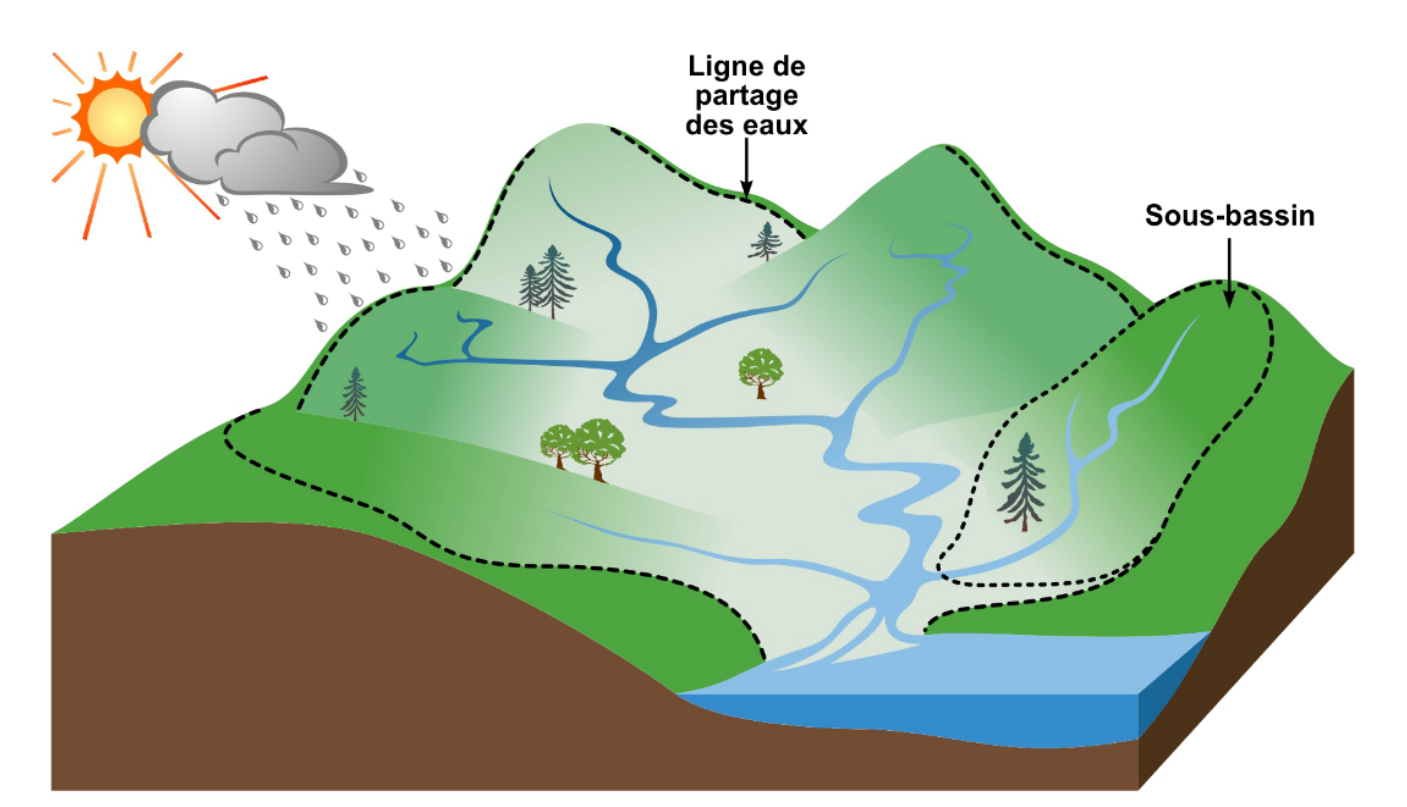
\includegraphics[scale=0.15]{bassin_versant.png}
		\captionof{figure}{Bassin versant (Source :http://rqes-gries.ca/).}
	\end{center} 
	
	À l’échelle du bassin versant, on distingue deux types d’écoulements: les écoulements de subsurface, les écoulements de surface. 
	
	\textbf{Les écoulements de subsurface}:\\
	
	La notion d'écoulement de subsurface se rapporte à l'écoulement de l'eau dans les pores du sol. L'écoulement de subsurface dépends de plusieurs paramètres comme les caractéristiques du sol(la porosité, la perméabilité), la saturation en eau du sol la topographie et le climat (précipitation, évaporation, transpiration). Ces écoulements sont traités par les équations de la mécanique des fluides (voir section  à citer) et pour plus de détails \cite{de1986quantitative}. 
	
	\textbf{Les écoulements de surface:}\\
	
	Les écoulements de surface, aussi qualifiés de ruissellement, sont la conséquence de deux phénomènes distincts. Le ruissellement peut apparaître lorsque le sol est saturé en surface. En effet, lorsque le sol est saturé, l’eau ne peut s’y infiltrer \cite{cappus1960etude}. Cette condition de saturation à la surface du sol peut être la conséquence d'une nappe affleurant la surface, la zone satisfaisant cette propriété est appelée zone de suintement. Cela arrive naturellement lors d'épisode pluvieux pour les nappes peu profondes. Le ruissellement peut aussi être causé par de fortes précipitations, ainsi le débit surfacique peut devenir supérieur à la quantité d'infiltration et ainsi créer un ruissellement (voir la figure). La quantité d'infiltration décroit exponentiellement lors d'évènements pluvieux \cite{horton1933role}.  
	
	\begin{center}
		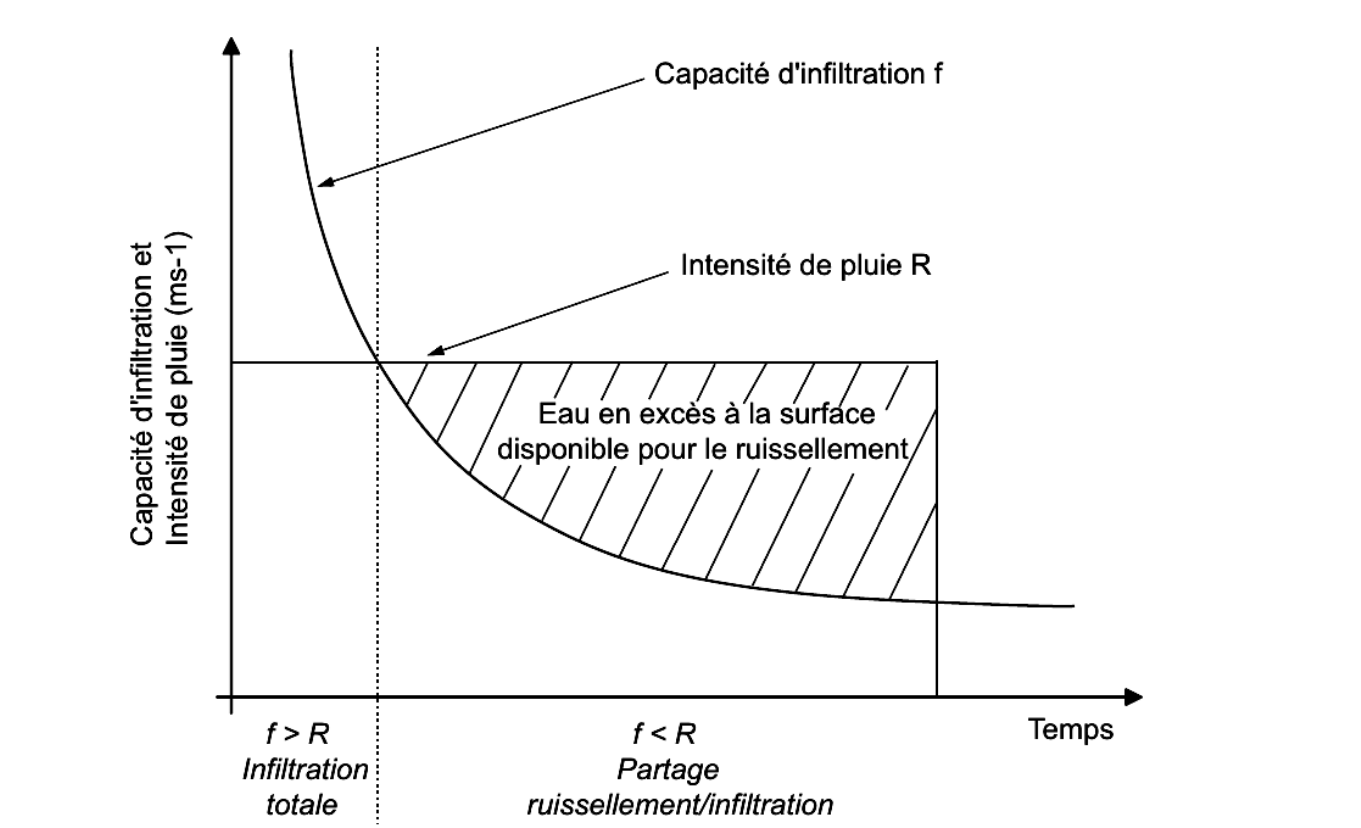
\includegraphics[scale=0.2]{ruissellement.png}
		\captionof{figure}{Estimation du ruissellement en fonction du temps modèle de Horton}
	\end{center} 
	
	\subsubsection{Transferts d'eau entre le sol et l'atmosphère}
	
	La végétation constitue le lien entre l'atmosphère et le sol. Les végétaux transfèrent de l'eau dans les deux sens, via les racines et la canopée. Il y a aussi des interactions directes entre le sol et l'atmosphère. Les trois principaux processus décrits sont l'évaporation du sol, la transpiration des végétaux ainsi que l'évaporation de l'eau interceptée par la canopée (mécanisme visant à conserver l'eau).\\
	
	\textbf{la transpiration:}\\
	
	La ``transpiration'' des plantes consiste en une libération de vapeur d’eau par les plantes dans l’atmosphère. Ce phénomène constitue une réponse passive à l’environnement atmosphérique dû à l’existence d’un gradient de pression positif de l’atmosphère à la canopée, on parle alors de demande atmosphérique. La description des processus d'évaporations ont été traités dans la thèse \cite{maquin2016developpement}.\\
	
	\textbf{Évaporation:}\\
	
	Sur les surfaces de sol non recouvertes de végétation (sol nu), l’eau présente dans le sol, à proximité de la surface, peut s’évaporer. Ce phénomène apparaît en présence d’un gradient de pression de vapeur d’eau entre le sol et l’atmosphère et d’un apport d’énergie. L’évaporation effective dépend de l’état hydrique de la surface du sol, l’énergie pour extraire l’eau du sol augmentant à mesure que le sol s’assèche et des propriétés conductrices du sol (voir \cite{hillel2003introduction}). \\
	
	\textbf{Pertes par interception:}\\
	
	Lors d’un épisode pluvieux, une partie de l’eau incidente est interceptée par le feuillage. Il s’agit du phénomène dit d’interception. Cette eau présente sur la canopée peut ensuite s’évaporer directement. On désigne ce processus d’évaporation sur la canopée comme les pertes par interception. L’importance de ce flux d’eau dépend de l’ampleur du feuillage et de la capacité de stockage d’eau de la canopée, c’est-à-dire de l’épaisseur maximale de la lame d’eau par unité de surface de feuillage\\
	
	
	\textbf{l'évapotranspiration potentielle:}\\
	
	On désigne par « évapotranspiration potentielle » la quantité d’eau maximale que l’atmosphère peut extraire via les trois processus décrits précédemment. Elle correspond ainsi à la demande atmosphérique évoquée auparavant. L’évapotranspiration potentielle correspond à l’évaporation d’une surface saturée en eau. Elle dépend de paramètres atmosphériques comme l’humidité de l’air, le vent et la température. Ce taux potentiel a la propriété de majorer la somme des flux de transpiration, d’évaporation et des pertes par interception.
	
	\subsection{Les concepts hydrologiques}
	\label{hydro}
	
	Nous allons ici introduire les principale notions à l'étude hydrologique des sols. Plusieurs caractéristiques définissent un sol, mais avant d'étudier en détail ce qui définit un sol, il est important de comprendre que l'étude hydro d'un sol est simplement un bilan d'eau dans celui-ci. Il faut alors commencer par déterminer ce qui rentre et ce qui sort. L'estimation de ces quantités est l'objet d'étude du downscaling qui cherche à prévoir la précipitation et l'évapotranspiration (l'eau drainée par les plantes recouvrant la surface).
	
	\subsubsection{Quelques définitions}
	
	\label{modelisation}
	\begin{definition}
		On appelle \textbf{porosité totale $\omega$} la valeur définie par
		\begin{equation}
			\omega =\frac{\textrm{Volume des vides}}{\textrm{Volume total de la roche}}.
		\end{equation}
		On appelle aussi \textbf{indice des vides $e$} la valeur définie par 
		\begin{equation}
			e=\frac{\textrm{Volume des vides}}{\textrm{Volume du solide plein}}.
		\end{equation}
		On peut passe d'une formule à l'autre par la relation 
		\[e\omega=e-\omega,\]
		Mais l'on utilise toujours la notion de porosité en hydrologie. 
	\end{definition}
	L'on peut trouver des méthodes de mesure de la porosité d'un sol dans l'ouvrage (\cite{marsily_de1986quantitative}). On dit aussi que le sol n'est pas saturé lorsque l'eau n'a pas pris tout l'espace disponible, on parle alors de saturation volumique.
	\begin{definition}
		On parle de \textbf{saturation volumique $\theta$}, la saturation définie par le rapport
		\begin{equation}
			\theta= \frac{\textrm{Volume d'eau contenu}}{\textrm{Volume total}},
		\end{equation}
		on a $0\leq<\theta\leq \omega$. Et la \textbf{saturation volumique $s$}
		\begin{equation}
			s=\frac{\textrm{Volume d'eau contenu}}{\textrm{Volume total des pores}}.
		\end{equation}
	\end{definition}
	
	En fonction de la saturation volumique les échelles de temps et les forces misent en action ne sont pas les mêmes.
	
	
	\subsubsection{Les équations pour modéliser l'écoulement}
	\label{darcy}
	On commence par rappeler les équations essentielles à la dynamiques des fluides. 
	L'équation de de conservation de la matière:
	\begin{equation}
		\label{cons-mat}
		div(\rho \overrightarrow{u})+\frac{\partial \rho}{\partial t}=0.
	\end{equation}
	Où $\rho$ est la masse volumique et $\overrightarrow{u}$ le vecteur vitesse du fluide. On écrit maintenant l'équation de Navier-Stokes
	\begin{equation}
		\frac{\partial p}{\partial x^i}-(\zeta+\frac{\mu}{3})\frac{\partial}{\partial x^i}(div\overrightarrow{u}) - \mu \nabla^2u^i=\rho(F^i -\frac{du^i}{dt}),
	\end{equation}
	$\zeta$ coefficient de viscosité du volume, (très souvent négligeable de vant $mu$) $[ML^{-1}T^{-1}]$,\\
	$\mu$ coefficient de viscosité dynamique, $[ML^{-1}T^{-1}]$\\
	$\nabla^2$ le laplacien,\\
	$F^i$ composante des forces à distance par unité de masse,\\
	$i$ un vecteur unitaire de l'espace $3D$.
	
	En milieu poreux les équations de Navier-Stokes deviennent difficilement applicables car le milieu dans lequel s'écoule le fluide dépend lui-même de l'écoulement du fluide. On donne des hypothèse simplificatrices pour résoudre l'équation de Navier-Stokes. 
	
	\noindent \textbf{Hypothèses simplificatrice:}\\
	En milieu poreux on peut émettre de nombreuses hypothèses simplificatrices qui permettent de simplifier l'équation de Navier Stokes, on commence par supposer les écoulement permanents
	\[\frac{\partial u^i}{\partial t}=0,\]
	on suppose aussi que le fluide est incompressible ($\rho$ constant) alors
	\[div(\rho \overrightarrow{u})=-\frac{\partial \rho}{\partial t}=0,\]
	et finalement,
	\[div \overrightarrow{u}=0.\]
	Dans ces hypothèses l'équation de Navier-Stokes devient
	\begin{equation}
		\frac{\partial p}{\partial x^i}-\mu \nabla^2u^i-\rho F^i=0. 
	\end{equation}
	
	Plusieurs méthodes numériques permettent de trouver des solutions à ce problèmes notamment la méthode de Galerkine ou les méthodes de différences finies voir \cite{allaire2005analyse} (chap 2, chap 6). 
	
	\vspace{7mm}
	Remarquons que ces équations ne prennent pas en compte la porosité du milieu, l'équation \eqref{cons-mat} peut être modifié en prenant en compte $\omega$ le coefficient de porosité et un terme source $q$ lié à la matière créant des interstices sans fluide (le coefficient est compté négativement). Alors l'équation de conservation s'écrit finalement
	\begin{equation}
		\label{eq-mass-por}
		div(\overrightarrow{U})+\frac{\partial}{\partial t}(\theta)+ q=0.
	\end{equation}
	Remarquons que l'on considère la porosité $w$ comme continue nous étudions des éléments de longueures $dx$ suffisamment petite pour que les équations de continuité soient considérée vrais et suffisamment grandes pour que l'on puisse considérer une porosité moyenne dans un élément de volume.
	
	\subsubsection{La loi de Darcy et l'équation de diffusivité en milieu poreux}
	\label{Darcy}
	Henry Darcy alors qu'il étudiait les fontaines de la ville de Dijon (1856) établit expérimentalement que le débit d'eau s'écoulant à travers un massif de sable peut se calculer
	\begin{equation}
		Q=KA\frac{\Delta h}{L}.
	\end{equation}
	$A$ est la section du massif sableux\\
	$\Delta h$ la perte de charge de l'eau entre le sommet et la base du massif sableux\\
	$K$ est une constante dépendant du milieu poreux, baptisée coefficient de perméabilité\\
	$L$ est l'épaisseur du massif sableux.
	
	On appelle $U=Q/A$ \textbf{la vitesse de filtration} d'un sol. À partir des équations de Navier-Stokes on sait que les causes du déplacement du fluide sont dûs au gradient de pression ainsi qu'aux forces extérieures. La loi de Darcy peut alors s'exprimer sous la forme générale
	\begin{equation}
		\label{eq-Darcy}
		\overrightarrow{U}=\frac{k}{\mu }(\overrightarrow{\nabla}\, p+\rho g \,\overrightarrow{\nabla}\, z).
	\end{equation} 
	On peut réécrire cette équation
	\[\overrightarrow{U}=-K(\overrightarrow{\nabla}\, h + \,\overrightarrow{\nabla}\, z),\]
	avec $K=k(\mu \rho g)^{-1}$ $[LT^{-1}]$ et $h=p(\rho g)^{-1}$ $[L]$. En posant 
	\[H=h+z,\]
	on peut alors injecter l'équation de Darcy \eqref{eq-Darcy} dans l'équation de conservation de la masse \eqref{eq-mass-por} pour finalement obtenir
	\begin{equation}
		\label{eq-Richards}
		-\overrightarrow{\nabla} \cdot (K\overrightarrow{\nabla}H)+\frac{\partial\theta}{\partial t}+ q=0.
	\end{equation}  
	On définit parfois des lois de porosité liées à la grandeur $f(H)=\theta$ la quantité d'eau est liée à la côte piézométrique et l'on pose 
	\[S_s(H)\frac{\partial H}{\partial t}=\frac{\partial\theta}{\partial t},\]
	$S_s$ est appelé le coefficient d'emmagasinement. On appelle l'équation ainsi obtenu en injectant la formule sur la porosité, \textbf{l'équation de Richard généralisée}
	\begin{equation}
		\label{eq-ge-richard}
		S_s(H)\frac{\partial H}{\partial t}-\overrightarrow{\nabla} \cdot (K(\theta)\overrightarrow{\nabla}H)+q=0.
	\end{equation}
	
	Ceux sont avec ces équations que les géologues travaillent, nous pouvons remarquer que cette simplification des équations peut être considérée comme un processus d'upscaling. Notons que les équations de Darcy ont été justifiées dans les travaux de Matheron et Marle à partir de l'intégration dans un milieu réel des équations de Navier. 
	
	
	\subsection{Les modèles}
	Il existe plusieurs modèles permettant de prédire les écoulements d'eau. Les premiers modèles sont les modèles de surface continentaux, ces modèles sont très complets et assurent une grande précision dans les résultats obtenus. Leurs temps de calcul les rendent inutilisables sur des grands domaines. On utilise alors des modèles moins complets mais aussi moins coûteux c'est le cas du modèle Orchidée 
	
	\subsubsection{Modèle de surface continentale Orchidée}
	
	Il s’agit d’un modèle dynamique, développé à l’échelle globale simulant les processus continentaux à partir des interactions sol-végétation-atmosphère. Ses résultats sont intégrés comme condition à la limite basse du modèle général de circulation atmosphérique du Laboratoire de Météorologie Dynamique (modèle LMDZ). Il modélise les interactions entre surface continentale et atmosphère, en particulier les flux d'énergie, d'eau et de carbone.
	
	
	\section{Prédictions climatiques}
	
	L'étude que nous avons menée a été réalisée sur le bassin du Little Washita. Nous avons eu accès à aux données NARR de $1979$ à $2014$.
	\subsection{Les données NARR et la méthodologie}
	\label{NARRs}
	Les données NARR (North American Regional Reanalysis) couvrent l'entièreté du continent nord américain. La méthode de projection pour passer de $\mathcal{S}(\mathbb{R}^3)$ à $\mathbb{R}^2$ est ce qu'on appelle la \textbf{projection Lambert}. Cette projection d'après le théorème de Gauss ne pas être une isométrie, cependant nous verrons que l'on pourra faire l'approximation que la géométrie obtenue est encore euclidienne pour le bassin du Washita et ses alentours (voir \ref{proj-Lambert}). Dans notre étude nous ferons comme si nous étions dans $\mathbb{R}^2$ en considérant le maillage carré, la longueur de grille du maillage est d'une trentaines de kilomètres (voir figure 1).
	
	
	Afin de déterminer l'efficacité du downscaling dans le cas où l'on ajoute du bruit à la variable que l'on cherche à prédire nous avons dégradé spatialement nos données en moyennant sur différentes échelles de grille.
	Nous les avons ensuite downscalées et puis les avons injectées dans un modèle hydrologique (voir à citer) et nous avons finalement comparé les résultats à partir des méthodes expliquées dans la section \ref{analyse-pred}.
	
	
	\begin{center}
		\label{maillage NARR}
		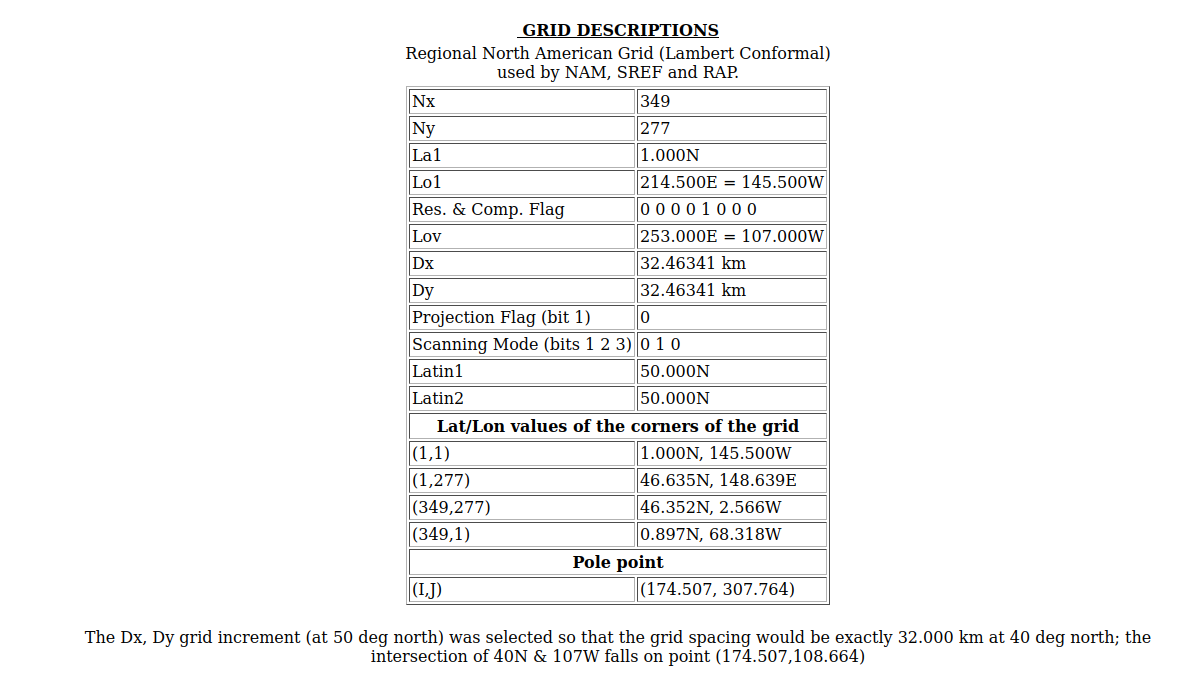
\includegraphics[scale=0.4]{grid_prop.png}
		\captionof{figure}{Description du maillage NARR}
	\end{center} 
	
	\subsection{Analyse de la structure spatiale des données NARRs}
	\label{spat-NARR}
	
	Nous avons considéré les coordonnées du Little Washita à $34.981^{\circ}N,-97.859^{\circ}W$. Nous repérons les coordonnées du point sur le maillage NARR étant le plus de ces coordonnées pour définir le point correspondant au Little Washita, en effet l'échelle du maillage NARR correspond à l'échelle du Little Washita, cette hypothèse est déjà faite dans la thèse \cite{maquin2016developpement}. 
	
	On commence par regarder les résultats autour du bassin du little washita, on fait un moyennage des précipitations et de l'évaporation sur un carré autour du little washita, le point de coordonnée (0,0) est le point correspondant au Little Washita sur ces figures. 
	
	\begin{figure}[h]
		\begin{minipage}[b]{0.48\linewidth}
			\centering 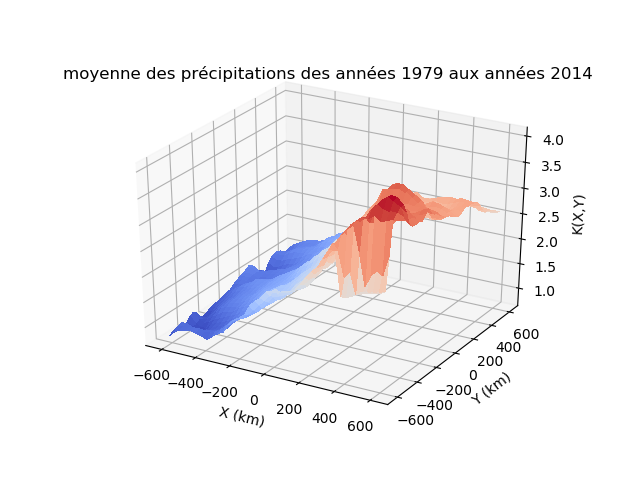
\includegraphics[scale=0.5]{images/mean_precip.png}
		\end{minipage}\hfill
		\begin{minipage}[b]{0.48\linewidth}	
			\centering 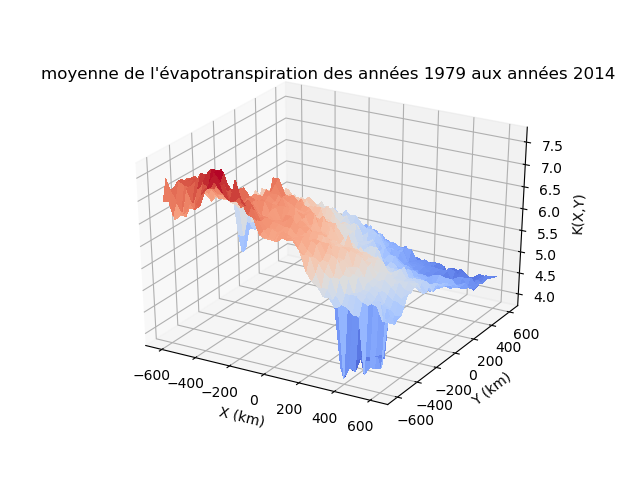
\includegraphics[scale=0.5]{images/mean_evap.png}
		\end{minipage}
	\end{figure} 
	
	Comme nous faisons une dégradation spatiale, il est intéressant comprendre la structure spatiale des données. Nous avons une grille spatiale pour laquelle nous avons vu que la géométrie pouvait être considérée comme euclidienne (voir \ref{proj-Lambert}). Les données NARRs que nous manipulons se présentent sous la forme d'un tenseurs $\mathcal{T}$ de dimensions $T \times M\times N\times v$ où $T$ est le nombre de jours sur lesquels ont a ces observations, $(M+1)\times (N+1)$ la dimension de la grille d'observation et $v$ le nombre de variables observées. Nous faisons l'hypothèse la fonction $S_{V}$ possède un noyau de covariance spatial $K$ et nous chercherons à déterminer sa forme. 
	
	\begin{definition}
		Soit $f:\mathbb{R}^{+}\times\mathbb{R}^2\to \mathbb{R}$ une fonction aléatoire, on définit un noyau de covariance sur cette fonction en faisant l'hypothèse que $f$ est stationnaire en temps et espace, on a alors
		\[Cov(f(t,x),f(t,x+y))=K(y), \hspace{4mm} \forall t \in \mathbb{R}^{+},\,x,y \in \mathbb{R}^2. \] 
	\end{definition}
	On remarque de plus que la fonction $K$ ainsi définie est symétrique, $K(y)=K(-y),\, \forall y \in \mathbb{R}^2$. On peut alors simplement calculer la covariance empirique à partir de l'estimateur sans biais de la variance.
	
	\[K(m,n)=\frac{1}{T(M-m+1)(N-n+1)-1}\sum_{t=1}^{T}\sum_{i=m}^{M}\sum_{j=n}^{N}(\mathcal{T}_{t,i,j}-\overline{\mathcal{T}}_{1,m,n})(\mathcal{T}_{t,i-m,j-n}-\overline{\mathcal{T}}_{2,m,n}),\]
	où,
	\[\overline{\mathcal{T}}_{1,m,n}=\frac{1}{T(M-m+1)(N-n+1)}\sum_{t=1}^{T}\sum_{i=m}^{M}\sum_{j=n}^{N}(\mathcal{T}_{t,i,j}), \hspace{4mm}\overline{\mathcal{T}}_{2,m,n}=\frac{1}{T(M-m+1)(N-n+1)}\sum_{t=1}^{T}\sum_{i=0}^{M-m}\sum_{j=0}^{N-n}(\mathcal{T}_{t,i,j}).\]
	On peut donc tracer le noyau de covariance $K(i,j)$, $i \in\{-N/2,N/2\}$, $j \in \{-M/2,M/2\}$. 
	
	\noindent \textbf{Résultats:}
	
	Pour obtenir nos résultats, nous avons pris en compte la saisonnalité. En effet, les résultats ont été obtenus sur chaque mois. Voici les résultats obtenus en fonction de la saisonnalité.
	
	\hspace{-3cm}
	\begin{tabular}{ccc} 
		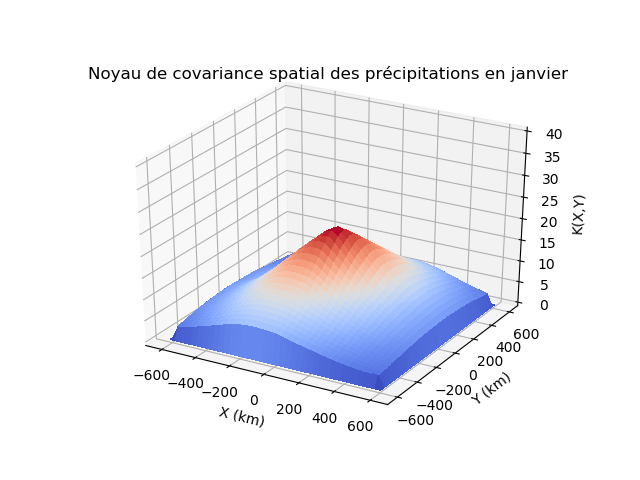
\includegraphics[scale=0.4]{images/kernel_precip_m1.png} & 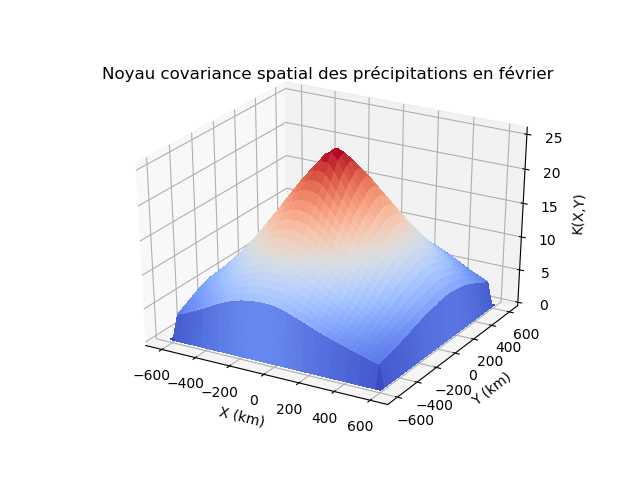
\includegraphics[scale=0.4]{images/kernel_precip_m2.png} & 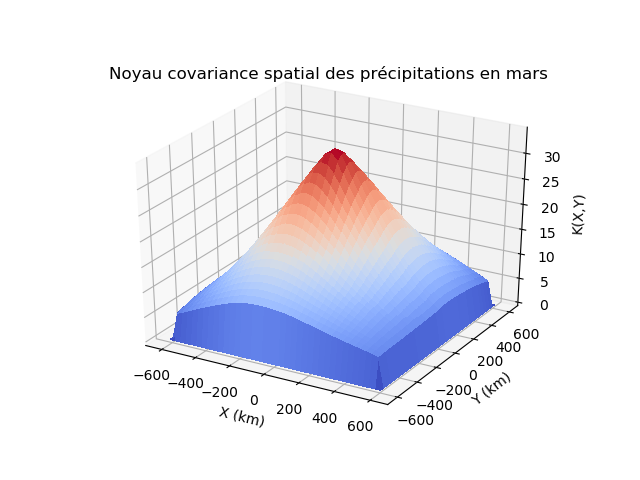
\includegraphics[scale=0.4]{images/kernel_precip_m3.png} \\ 
		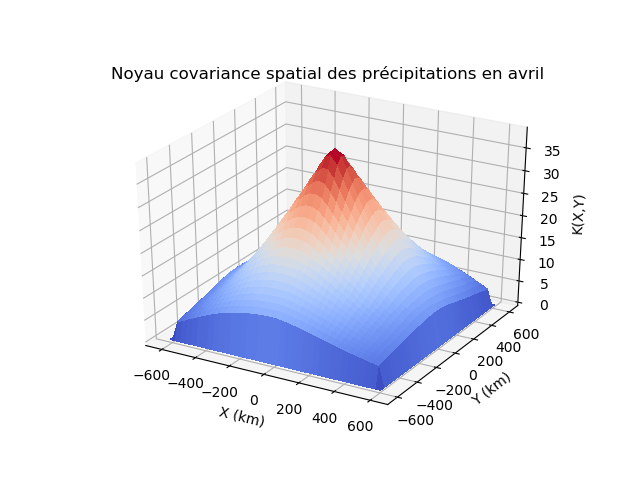
\includegraphics[scale=0.4]{images/kernel_precip_m4.png} & 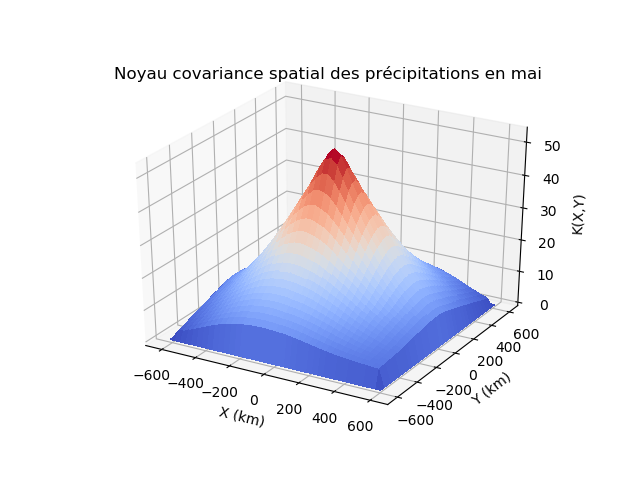
\includegraphics[scale=0.4]{images/kernel_precip_m5.png} & 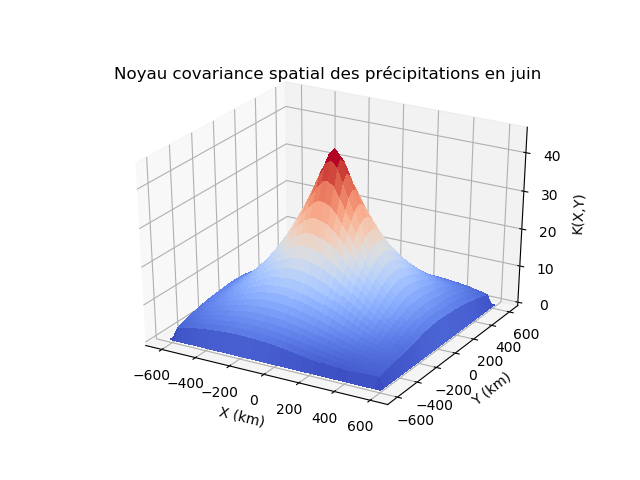
\includegraphics[scale=0.4]{images/kernel_precip_m6.png} \\
		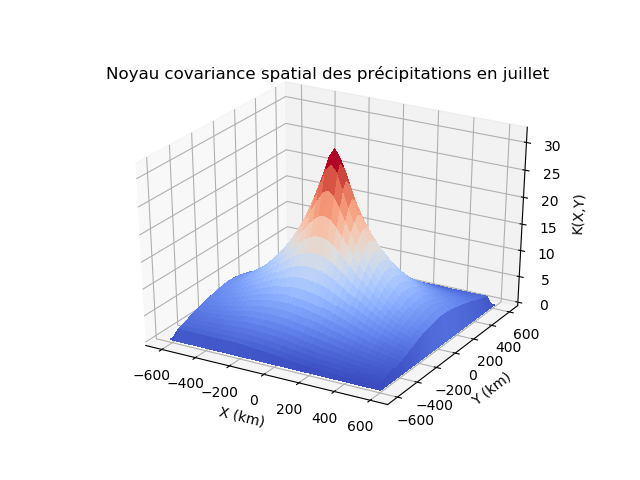
\includegraphics[scale=0.4]{images/kernel_precip_m7.png} & 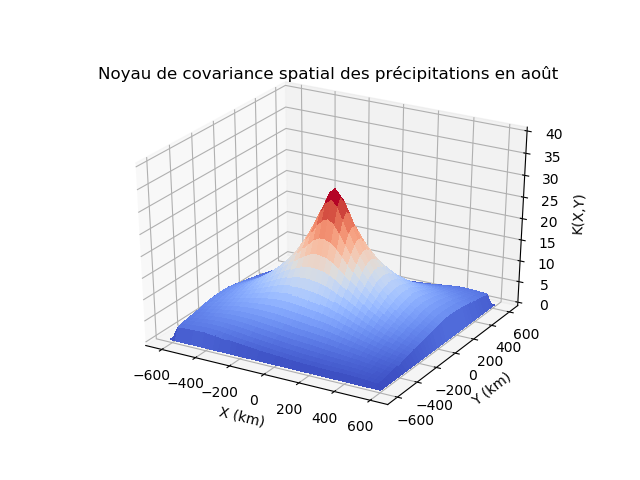
\includegraphics[scale=0.4]{images/kernel_precip_m8.png} & 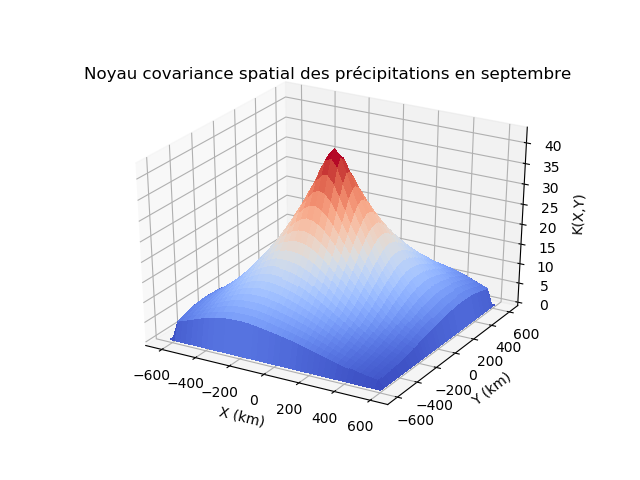
\includegraphics[scale=0.4]{images/kernel_precip_m9.png} \\ 
		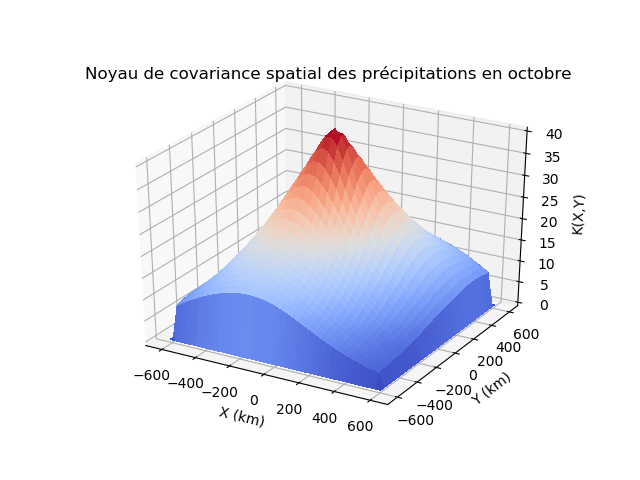
\includegraphics[scale=0.4]{images/kernel_precip_m10.png} & 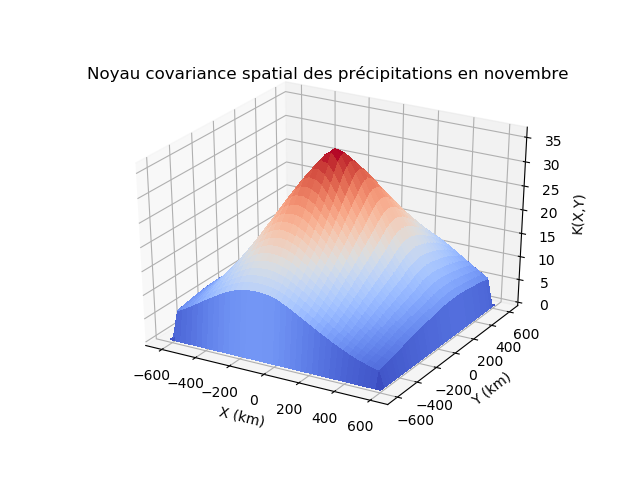
\includegraphics[scale=0.4]{images/kernel_precip_m11.png} & 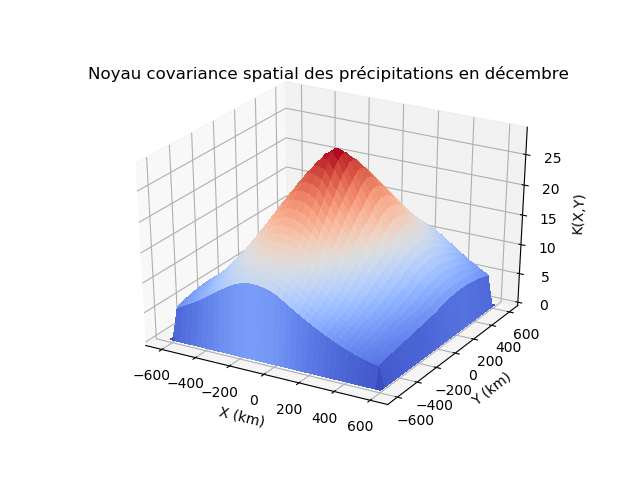
\includegraphics[scale=0.4]{images/kernel_precip_m12.png} \\
	\end{tabular} 
	
	Rappelons que l'axe $X$ correspond aux latitudes et l'axe $Y$ aux longitudes. Nous voyons qu'en été la covariance entre deux points s'effondre relativement vite alors qu'en hiver c'est plutôt l'inverse.
	Il semble intéressant de remarquer l'odre d'échelle à partir du quel les variables sont décorélées, en effet même si l'on est à plusieurs centaines de kilomètres d'un point, on observe encore une covariance positive, on pourrait s'attendre à ce que ca s'effondre beaucoup plus vite. Cependant ces résultats semblent indiquer qu'il y a une forte corrélation spatiale pour la précipitation et l'évapotranspiration. On peut aussi remarque qu'en hiver il semble très important que la covariance selon les longitudes s'effondre moins vite que selon les latitudes. Alors qu'en été on peut voir quasiment faire l'hypothèse que $K(y)=K(\|y\|)$. 
	
	\subsection{Présentation des résultats de prédictions climatiques}
	\label{ch pr-res-clim}
	Nous allons travailler avec plusieurs séries temporelles différentes. Nous aurons la série de référence $Y$ issue des réanalysis des données récoltées sur le Little Washita de $1979$ à $2014$, puis nous aurons les séries dégradées spatialement et une série issue du modèle de climat de l'IPSL.
	
	On commence par réintroduire le tenseur $\mathcal{T}$ de dimension $T \times M\times N$. Nous pouvons exprimer données NARRs par un tenseur. 
	\[\mathcal{T}_{t,m,n}=\mathcal{T}_V(t,lat_m,lon_n).\]
	où $t$ correspond à un temps et $(m,n)$ à une position.
	
	\subsubsection{La dégradation}
	\label{ch deg-spat}
	
	Nous avons dégradé les valeurs par un moyennage spatial. Nous avons fait $4$ dégradations différentes nous allons les numéroter ainsi $\{1,2,3,4\}$ et on appellera $\mathcal{T}^{d}$ le tenseur issu de la dégradation $d$, défini par
	\begin{equation}
		\label{eq-degradation}
		\mathcal{T}^{d}{t,m,n}=\frac{1}{(2d+1)^2} \sum_{i=-d}^{d}\sum_{j=-d}^{d}\mathcal{T}_{t,m+i,n+j} \hspace{4mm} \forall (m,n) \in \{d+1,...,M-d\}\times\{d+1,...., N-d\}. 
	\end{equation}
	
	Nous avons alors étudié le point correspondant au bassin du Little Washita de coordonnées $(a,b)$ et l'on appellera, $(X^d_t)_{t\in \llbracket 1,T \rrbracket}$ les séries temporelles $\mathcal{T}^{d}{t,a,b}$. Nous avons cherché à prédire la série $(Y_t)_{t \in \llbracket 1,T \rrbracket}= \mathcal{T}^{0}{t,a,b}$ à partir des séries $(X^d_t)_{t\in \llbracket 1,T \rrbracket}$ et ainsi regarder l'impacte de la dégradation puis du downscaling sur les données.
	
	\subsection{Les résultats de la dégradation et du downscaling sur les données}
	Nous allons utiliser les outils définis dans la section \ref{analyse-pred} pour analyser la qualité de nos prédictions.
	
	\subsubsection{tracé des boxplot}
	
	Nous avons tracé les boxplot des précipitations et de l'évapotranspiration afin de voir visuellement répartitions des points.
	
	
	\hspace{-1cm}
	\begin{tabular}{ccc}
		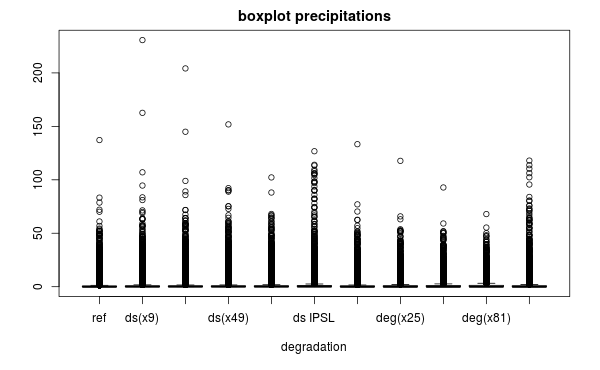
\includegraphics[scale=0.4]{images/boxplot_precip.png} & 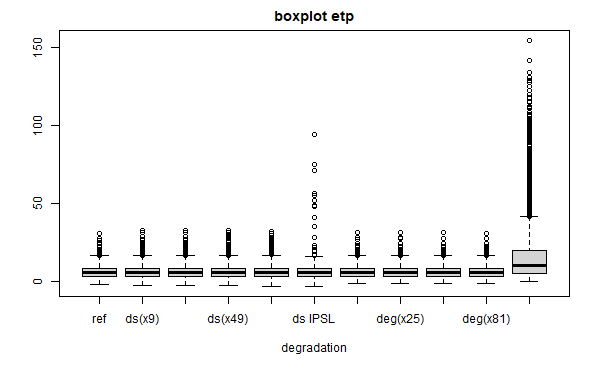
\includegraphics[scale=0.4]{images/boxplot_evap.png}   \\
	\end{tabular} 
	
	On voit que la dégradation de l'évapotranspiration n'a quasiment aucune influence sur les séries temporelle, ce qui été à prévoir d'après le noyau de covariance que nous obtenu précédemment. On peut aussi voir que le modèle de climat de l'IPSL prédit relativement mal l'évapotranspiration sur la région du Little Washita. On peut aussii voir la méthode de prédiction utilisée pour downscaler les série temporelles dégradées est la méthode  \textbf{CDF-t avec support égale}. 
	
	\subsubsection{affichage des données prédites en fonction des données réelles}
	
	On commence par afficher les résultats sur un graphique en mettant les données de précipitation prédites en fonction des données de précipitation réelles, cette méthode permet de juger visuellement de l'efficacité du downscaling sur les données. Les figures qui affichées indiquent le degrée de déformation dans leur titre sous la forme $(2d-1)^2$ où $d$ est le degrés que celui de l'équation \eqref{eq-degradation}. L'on peut voir sur chaque ligne à droite les données dégradées et à gauches les mêmes série après avoir appliquer un downscaling sur ces données.
	
	\hspace{-1cm}
	\begin{tabular}{c} 
		\includegraphics[scale=0.4]{images/pr_ 1 _ds.png} & \includegraphics[scale=0.4]{images/pr_ 1 _dg.png}  \\ 
		\includegraphics[scale=0.4]{images/pr_ 2 _ds.png} & \includegraphics[scale=0.4]{images/pr_ 2 _dg.png}  \\
	\end{tabular}
	
	\hspace{-1cm}
	\begin{tabular}{c}
		\includegraphics[scale=0.4]{images/pr_ 3 _ds.png} & \includegraphics[scale=0.4]{images/pr_ 3 _dg.png}   \\
		\includegraphics[scale=0.4]{images/pr_  4 _ds.png} & \includegraphics[scale=0.4]{images/pr_ 4 _dg.png}  \\
	\end{tabular}
	
	Visuellement il semble que le downscaling améliore les prédictions. Nous avons tracé pour chaque figure en noir la droite identité et en rouge les droites de régression linéaire de la forme $y=ax+b$, où $y$ est la précipitation de référence et $x$ le prédicteur de $y$ dans notre cas c'est soit la dégradation $\mathcal{T}_{d,a,b}$ soit son downscalé à partir de la méthode définie dans la section \ref{CDf-t-algo}. Remarquons que la dégradation de nos données ne crée pas de changement important de l'éparpillement des points dans les graphiques, c'est en accord avec les figures obtenues dans la section \ref{spat-NARR} montrant une grande corrélation spatiale. Il semble cependant que la dégradation ait une tendance à sous-évaluer les précipitations élevées, ce qui ne semble pas abérrant si l'on considère les tailles des cumunolimbus (allant de $2$ à $10$km ), inférieur à la largeur de grille des données NARRs ($32$km). 
	
	\subsubsection{Différence analyse Root Mean Square error et distance de Cramér-von Mises}
	
	Nous avons calculer la distance quadratique moyenne entre la série de référence et les différentes séries de dégradation. Les résultats ainsi obtenues sont:
	
	\vspace{0.5cm}
	
	\hspace{-1cm}
	\begin{tabular}{ccc}
		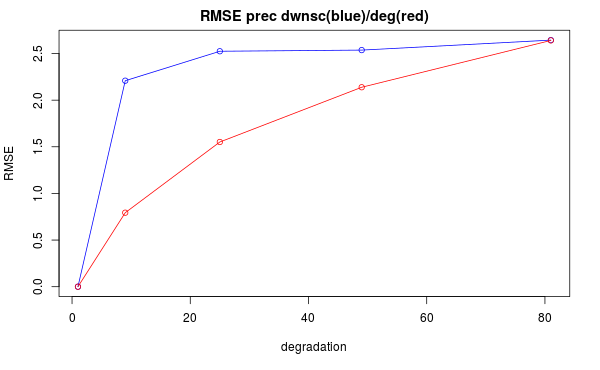
\includegraphics[scale=0.4]{images/RMSE_precip.png} & 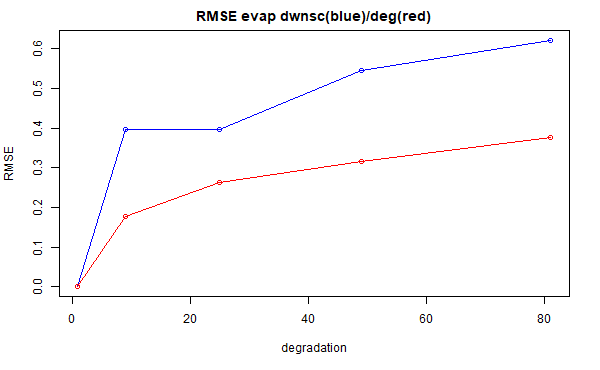
\includegraphics[scale=0.4]{images/RMSE_evap.png}  \\
	\end{tabular} 
	
	Nous voyons que les résultats sont mauvais, mais encore une fois, ce n'est pas cette distance que nous cherchons à minimiser avec le downsaling, mais une distance sur les fonctions de répartition. Regardons maintenant la distance de Cramér-Von Mises.
	
	\vspace{0.5cm}
	
	\hspace{-1cm}
	\begin{tabular}{ccc}
		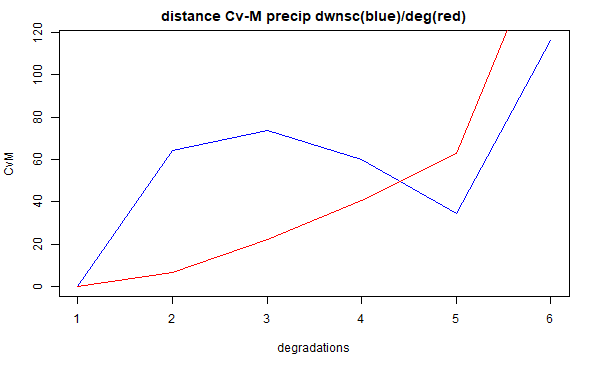
\includegraphics[scale=0.4]{images/Dist_CVM_precip.png} & 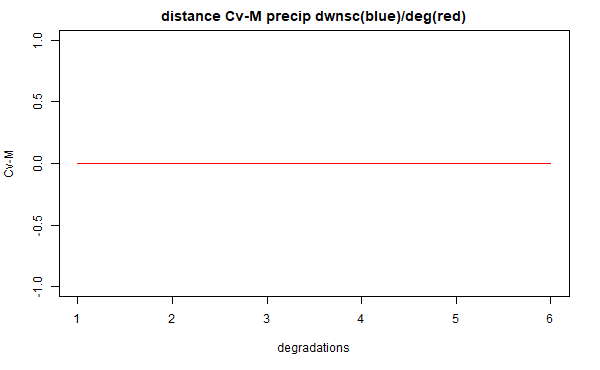
\includegraphics[scale=0.4]{images/Dist_CVM_evap.png}  \\
	\end{tabular} 
	
	
	L'on voit qu'encore une fois la prédiction après downscaling est plus mauvaise que seulement la série dégradée, jusqu`à la dégradation $d=5$ et $d=6$ sont les données $IPSL$. L'algorithme effectue alors une grosse correction pour ce cas-ci. Cette erreur de prédiction soulève un point que nous n'avons pas encore abordé jusqu'à présent, c'est le fait que notre échantillon de précipitation possède de nombreuses valeurs à $0$, ce qui signifie que la densité n'est plus une fonction mais un distribution avec un poids non nul en $0$. C'est ce détail qui crée cette différence, si l'on enlève les précipitations nulle, nous obtenons:
	
	\vspace{0.5 cm}
	
	\hspace{-1cm}
	\begin{tabular}{ccc}
		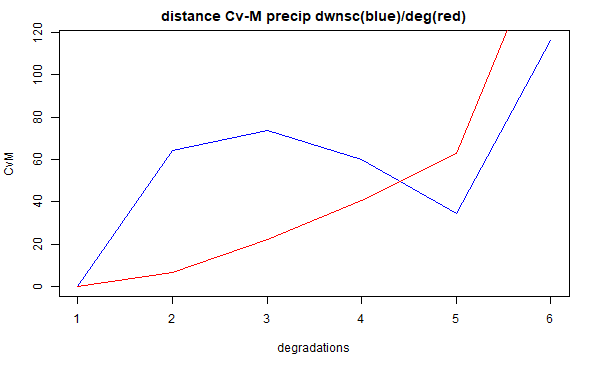
\includegraphics[scale=0.4]{images/Dist_CVM_precip.png} & 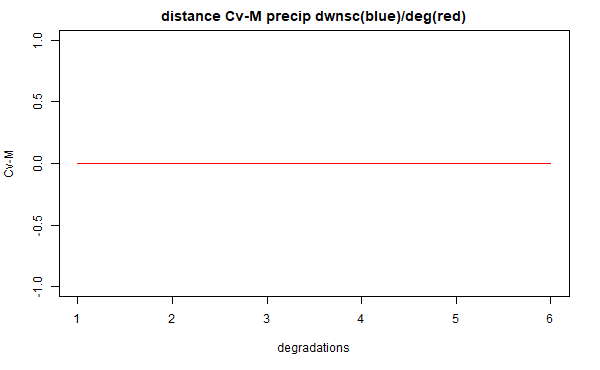
\includegraphics[scale=0.4]{images/Dist_CVM_evap.png}  \\
	\end{tabular} 
	
	
	
	
	\section{Indexes}
	
	\subsection{Indexe \ref{C-v} : La statistique de Cramér-von Mises}
	\label{lemme Cramer-von Mise}
	Soient $(X_i)_{i\in \llbracket 1,n \rrbracket}$ et $(Y_i)_{i\in \llbracket 1,m \rrbracket }$ des réalisations indépendante issues de variables aléatoires réelles $X$ et $Y$. On appelle $\mathcal{F}_{n}$ et $\mathcal{G}_{m}$ les fonctions de répartitions empiriques définie à partir de ces réalisation et $\mathcal{H}_{m,n}$ la fonction de répartition empirique définie à partir de l'ensemble de ces réalisations $(Z_i)_{i\in \llbracket 1,m+n \rrbracket }=X_1,...,X_n,Y_1,...,Y_m$. Par la suite on considéra que tous les éléments sont triés dans leur ensemble ($i\leq j \Rightarrow E_i\leq E_j$). Nous avons alors l'égalité suivante
	\begin{equation}
		C_{n,m}=\frac{nm}{n+m}\int_{\mathbb{R}}\big[ \mathcal{F}_{n}(x)-\mathcal{G}_{m}(x)\big]^{2} \mathrm{d} \mathcal{H}_{m,n}(x)=\frac{1}{nm(m+n)}\Big[ n\sum_{i=1}^{n}(R_{X_i}-i)^2+ m\sum_{i=1}^{m}(R_{Y_i}-i)^2\Big]-\frac{4nm-1}{6(m+n)}.
	\end{equation}
	où $R_{X_i}$ est le rang de $X_i$ dans $X_1,...,X_n,Y_1,...,Y_n$ autrement dit 
	\[R_{X_i}=Card(\{j \in \llbracket 1,m+n \rrbracket , Z_j\leq X_i\}).\] 
	Notons que cette égalité transforme un problème d'analyse en un problème de dénombrement beaucoup plus simple. On rappelle la définition de l'intégrale par rapport à une fonction.
	\begin{definition}
		Soient $f$ une fonction continue par morceaux de $\mathbb{R}$ dans $\mathbb{R}$, soit $g$ une fonction continue par morceaux on définit l'intégrale en appelant $x_{i,n}=i/n$
		\[\int_{\mathbb{R}}f(x)\, dg(x)=lim_{n\to\infty}\sum_{i \in \mathbb{Z}}f(x_{i,n})\big( g\big(x_{i,n}\big)-g\big(x_{i,n-1})\big).\]
	\end{definition}
	
	\begin{proof}
		
		\noindent Commencons par montrer l'égalité
		\[\frac{nm}{n+m}\int_{\mathbb{R}}\big[ \mathcal{F}_{n}(x)-\mathcal{G}_{m}(x)\big]^{2} \mathrm{d} \mathcal{H}_{m,n}(x)=\frac{mn}{(m+n)^2}\sum_{i=1}^{m+n}\big(\mathcal{F}_n(Z_i)-\mathcal{G}_{m}(Z_i)\big)^2.\]
		On pose $\delta=\inf \{|Z_i-Z_j|, Z_i \neq Z_j\}$, quel que soit $n\geq n_0$ tel que $1/n_0< \delta$ on a: 
		\[\sum_{i \in \mathbb{Z}}\big(\mathcal{F}_n(\frac{i}{n})-\mathcal{G}_{m}(\frac{i}{n})\big)^2\Big( \mathcal{H}_{m,n}\big(\frac{i}{n}\big)-\mathcal{H}_{m,n}\big(\frac{i-1}{n}\big)\Big)=\sum_{i=1}^{m+n}\big(\mathcal{F}_n(Z_i)-\mathcal{G}_{m}(Z_i)\big)^2,\]
		on obtient donc directement l'égalité voulue en passant à la limite.
		
		Observons maintenant que $\mathcal{F}_n(X_i)=i/n$ et $\mathcal{G}_m(X_i)=(R_{X_i}-i)/m$ ainsi que $\mathcal{F}_n(Y_i)=(R_{Y_i}-i)/n$ et $\mathcal{G}_m(X_i)=i/m$. On peut alors réécrire $C_{n,m}$ en séparant la somme sur les $X_i$ et $Y_i$
		\[C_{n,m} = \frac{mn}{(m+n)^2}\Big[\sum_{i=1}^{n} \Big(\frac{i}{n}-\frac{R_{X_i}-i}{m}\Big)^2+ \sum_{i=1}^{m}\Big(\frac{R_{Y_i}-i}{n}-\frac{i}{m}\Big)^2 \Big]\]
		\[=\frac{mn}{(m+n)^2}\Big[\frac{1}{m^2}\sum_{i=1}^{n}\Big(R_{X_i}-i\frac{m+n}{n}\Big)^2 +
		\frac{1}{n^2}\sum_{i=1}^{m}\Big(R_{Y_i}-i\frac{m+n}{m}\Big)^2\Big]\]
		Remarquons que $C_{n,m}$ est de la forme
		\[C_{n,m}=\frac{mn}{(m+n)^2}\Big[\frac{C_1}{m^2}+\frac{C_2}{n^2} \Big],\]
		et que $C_1$ et $C_2$ sont symétriques en $n$ et $m$. On définit $\Sigma_1=\sum_{i=1}^{n}R^{2}_{X_i}$, $\Sigma_2=\sum_{i=1}^{m}R^{2}_{Y_i}$ et $\mathcal{S}_{k}=\sum_{i=1}^{k}i^2$ nous allons travailler sur l'expression
		\[C_1=\sum_{i=1}^{n}\Big(R_{X_i}-i\frac{m+n}{n}\Big)^2.\]
		On la développe puis factorise pour obtenir
		\[C_1=\frac{m+n}{n}\sum_{i=1}^{n}(R_{X_i}-i)^2-\frac{m}{n}\Sigma_1+\frac{m(m+n)}{n^2}\mathcal{S}_n.\]
		On obtient de la même manière
		\[C_2=\frac{m+n}{m}\sum_{i=1}^{m}(R_{Y_i}-i)^2-\frac{n}{m}\Sigma_2+\frac{n(m+n)}{m^2}\mathcal{S}_m.\]
		D'après ce qu'on a dit précédemment on a donc: 
		\[C_{n,m}=\frac{1}{nm(m+n)}\Big[ n\sum_{i=1}^{n}(R_{X_i}-i)^2+ m\sum_{i=1}^{m}(R_{Y_i}-i)^2\Big]-\frac{\Sigma_1+\Sigma_2}{(m+n)^2}+ \frac{\mathcal{S}_n}{n(n+m)}+ \frac{\mathcal{S}_m}{m(m+n)}.\]
		
		On remarque $\Sigma_1+\Sigma_2 = \mathcal{S}_{m+n}$ et que l'on a la première moitié de notre somme. 
		Il ne reste plus qu'à développer l'expression 
		\[-\frac{\mathcal{S}_{m+n}}{(m+n)^2}+ \frac{\mathcal{S}_n}{n(n+m)}+ \frac{\mathcal{S}_m}{m(m+n)}\]
		\[=-\frac{(m+n+1)(2m+2n+1)}{6(m+n)}+ \frac{(n+1)(2n+1)}{6(m+n)}+\frac{(m+1)(2m+1)}{6(m+n)}=-\frac{4mn-1}{6(m+n)}\]
		En regroupant nos deux résultats nous avons finalement:
		\[C_{n,m}=\frac{1}{nm(m+n)}\Big[ n\sum_{i=1}^{n}(R_{X_i}-i)^2+ m\sum_{i=1}^{m}(R_{Y_i}-i)^2\Big]-\frac{4nm-1}{6(m+n)}\]
	\end{proof}	
	
	\subsection{Indexe 2: Projection conique conforme de Lambert}
	\label{proj-Lambert}
	La plupart des fonctions de projection de $S(\mathbb{R}^3)$ dans $\mathbb{R}^2$ sont des surfaces développables sur lesquelles ont projette les points de la terre. Par exemple des cônes, des cylindres et des plans (projection stéréographique) sont les surfaces développable les plus connues. La \textbf{projection Lambert} est une projection cônique aussi appelée la projection orthomorphique. Ses caractéristiques sont décrites dans le livre \cite{grafarend2014map}. Elle possède la caractéristique de préserver les angles et les distances pour deux latitudes choisies, pour les données NARR les latitudes choisies sont $33^{\circ}$N et $45^{\circ}$N. De plus les lignes de latitudes égales sont des cercles et celles de longitudes égales des lignes droites. Les coordonées que nous étudions sont entre $33^{\circ}$N et $36^{\circ}$N. On va montrer que les longueures étudiées dans cette zone de l'espace ne souffrent que de très peu de déformation. 
	
	
	\begin{center}
		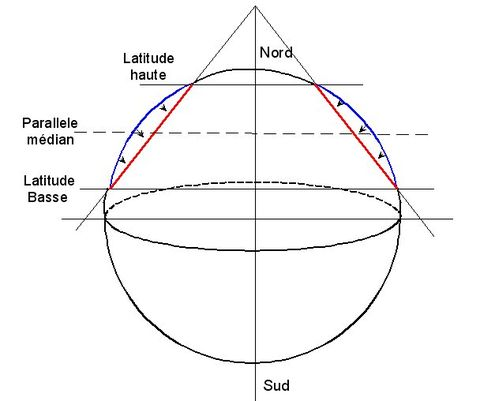
\includegraphics[scale=0.4]{lambert.jpg}
		\captionof{figure}{Projection conique conforme de Lambert}
	\end{center}
	
	\begin{definition}
		On définit les fonctions $lat:S(\mathbb{R}^3)\to [-\pi/2,\pi/2] $ et $lon:S(\mathbb{R}^3) \to [-\pi,\pi] $ qui associent à chaque point $x$ de $S(\mathbb{R}^3)$ sa latitude et sa longitude en radiant.
	\end{definition} 
	\begin{definition}
		On définit le cône convexe $\zeta_{\theta,\theta+\epsilon}$ comme l'ensemble des droites passant les points $x_1$ et $x_2$ de même longitudes de latitudes égale à $\theta$ et $\theta+\epsilon$. Autrement dit
		\[\zeta_{\theta,\theta+\epsilon}=\{D(x_1,x_2), \, x_1,x_2 \in S(\mathbb{R}^3), \, lon(x_1)=lon(x_2),\, lat(x_1)=\theta,\, lat(x2)=\theta+\epsilon\}.\] 
		où $D(x_1,x_2)$ est la droite passant par $x_1$ et $x_2$.
	\end{definition}
	
	
	Il est évident que pour les lignes de latitude haute ($\theta+ \epsilon$) et basse ($\theta$) les longueures sont conservées. On définit $\epsilon=\pi (45-33)/180$. 
	
	
	\begin{proposition}
		Pour toute courbe $\gamma: [0,1] \to S(\mathbb{R}^3)$ continue dont les latitudes sont comprises entre $\theta$ et $\theta+\epsilon$, on a 
		\[\min\Big(\cos(\epsilon/2),\frac{\cos(\theta+\epsilon)}{\cos(\theta)} \Big)\leq \frac{\|P(\gamma)\|_{\|\cdot\|_{\mathbb{R}^2}}}{\|\gamma\|_{\|\cdot\|_{S(\mathbb{R}^3)}}} \leq 1.\]
		Où $P$ est la projection de Lambert conservant les longueures pour les latitudes $\theta$ et $\theta+\epsilon$.
	\end{proposition} 
	Ce résultat permettra de conclure que la géométrie des lieux peux être considérée comme euclidienne si $\epsilon$ est suffisamment petit.
	
	\begin{proof} (Esquisse) On montrera cette inégalité pour les courbes de latitudes constantes et pour celles de longitudes constantes et la densité des fonctions de longitude ou de latitude par morceaux constantes dans l'ensemble des courbes permettra de conclure cette inégalité pour toutes les courbes.
		
		\vspace{4mm}
		
		On définit trois ensembles de courbes, $\mathcal{C}_1$, $\mathcal{C}_2$ et $\mathcal{C}_{m}$ tels que \[\mathcal{C}_1=\{\gamma \in \mathcal{C},\, lon(\gamma(t))=c, \, \forall t \in [0,1],\]
		\[\mathcal{C}_2=\{\gamma \in \mathcal{C},\, lat(\gamma(t))=c, \, \forall t \in [0,1]\},\]
		\[\mathcal{C}_m=\{\gamma \in \mathcal{C},\, \exists t_1<...<t_n,\forall \leq i<n, \gamma_i: t \mapsto \gamma(t_i+ t(t_{i+1}-t_i)) \in \mathcal{C}_1 \cup \mathcal{C}_2\}.\]
		On commence par étudier les courbes $\gamma$ dans $\mathcal{C}_1$ injectives, on peut alors sans perte de généralité se placer dans le cas du cercle unité dans $\mathbb{R}^2$ (le cercle de longitude constante). On a alors l'égalité
		
		\[\|\gamma\|_{\|\cdot\|_{S(\mathbb{R}^3)}}=\|\gamma\|_{\|\cdot\|_{S(\mathbb{R}^2)}}=\int_{0}^{1}|\gamma'(t)|dt.\]
		
		\begin{center}
			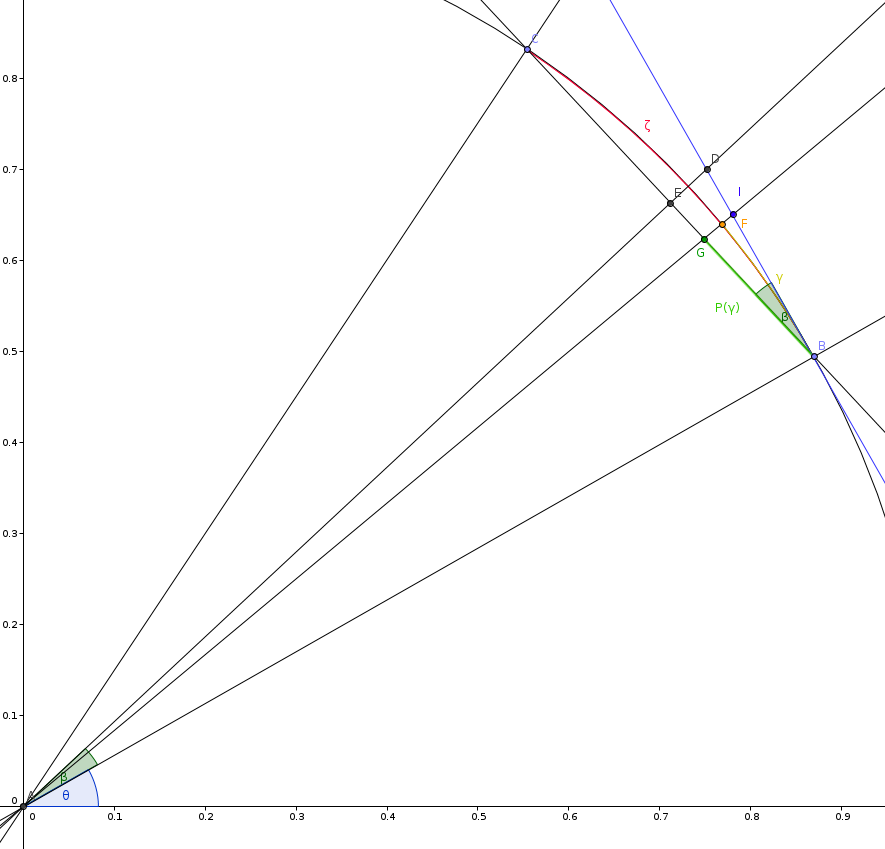
\includegraphics[scale=0.25]{images/geogebra_lambert.png}
			\captionof{figure}{Figure explicative de la projection lambert conformale}
		\end{center}
		D'après ce schéma, on voit que pour tout point $F$ sur le cercle la longueur de la courbe $\gamma$ allant de $B$ à $F$  est majorée par la longueur du segment $BI$, de plus sur la figure  on a $\epsilon/2=\beta$. On obtient facilement l'inégalité
		\[\cos(\epsilon/2)\leq\frac{\|P(\gamma)\|_{\|\cdot\|_{\mathbb{R}^2}}}{\|\gamma\|_{\|\cdot\|_{S(\mathbb{R}^3)}}},\]
		
		Étudions maintenant les courbes $\gamma$ dans $\mathcal{C}_2$ de latitude égale à $\theta+\epsilon$ et injectives. On sait que la courbe $\gamma$ ainsi que sa projection $P(\gamma)$ décrivent un arcs de cercle dans $\mathbb{R}^3$. Le rapport entre la longueur de l'arc de cercle définit par $P(\gamma)$ et $\gamma$ dans $\mathbb{R}^3$ est majoré grossièrement par $\cos(\theta+\epsilon)/\cos(\beta)$.
		\[\frac{\cos(\theta+\epsilon)}{\cos(\beta)}\leq\frac{\|P(\gamma)\|_{\|\cdot\|_{\mathbb{R}^2}}}{\|\gamma\|_{\|\cdot\|_{S(\mathbb{R}^3)}}}\]
		
		Pour chaque courbe $\gamma$ dans $\mathcal{C}_m$ on a alors 
		\[\min\Big(\frac{2\sin(\epsilon/2)}{\epsilon},\frac{\cos(\theta+\epsilon)}{\cos(\theta)} \Big)\leq \frac{\|P(\gamma)\|_{\|\cdot\|_{\mathbb{R}^2}}}{\|\gamma\|_{\|\cdot\|_{S(\mathbb{R}^3)}}} \leq 1,\]
		la densité de $\mathcal{C}_m$ dans l'ensemble des courbes continues permet de conclure.
	\end{proof}
	
	Finalement, on peut voir que dans notre cas où $\theta=\pi 33/180$ et $\epsilon=\pi 12/180$. On a que pour toute courbe $\gamma:[0,1]\to S(\mathbb{R}^3)$ dont la latitude est comprise entre $\theta$ et $\theta+\epsilon$ on a
	\[0.84\leq \frac{\|P(\gamma)\|_{\|\cdot\|_{\mathbb{R}^2}}}{\|\gamma\|_{\|\cdot\|_{S(\mathbb{R}^3)}}} \leq 1.\]
	
	\subsection{Indexe 3: Classification des populations de débit}
	On commence par rappeler ce que sont les données $\Delta Q$ et $\Delta R$, sont les différences entre les séries prédites et les séries de référence ($R$ correspond à la pluie et $Q$ au débit). Nous avons vu  que les schémas nous incitent à considérer deux classes de points (citer la partie correspondante).
	
	\begin{center}
		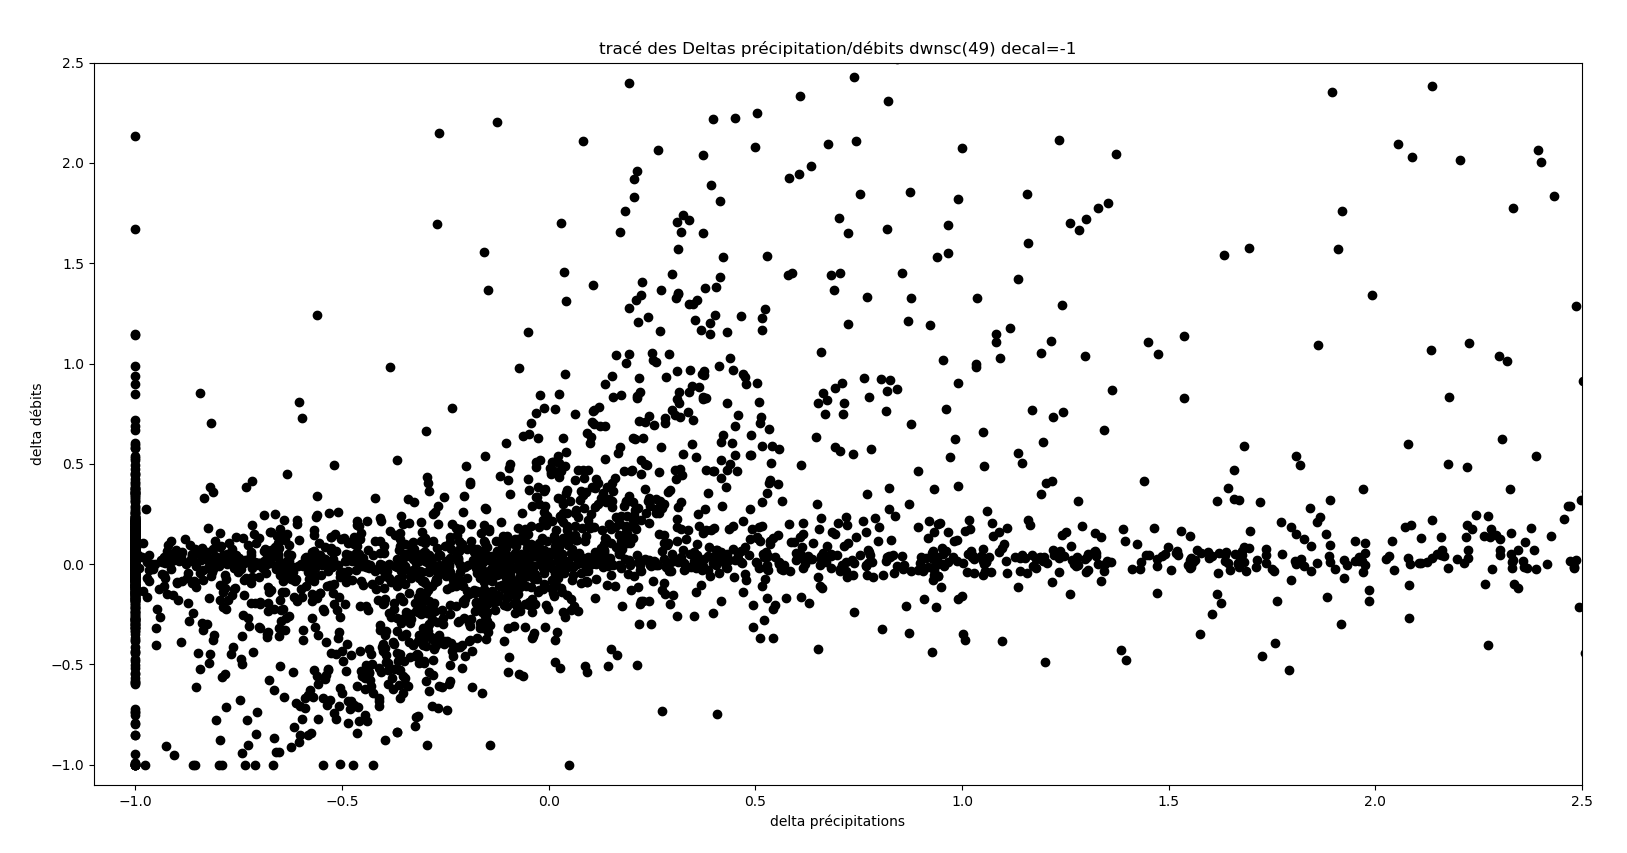
\includegraphics[scale=0.28]{images/deb_prec_dec1.png}
		\captionof{figure}{tracé des $\Delta Q(t)$ en fonction des $\Delta R(t-1)$}
	\end{center}
	On définit alors les ensembles $\mathcal{C}$ et $\mathcal{I}$ tels que
	\[\mathcal{C}=\{(\Delta Q(t),\Delta R(t-1)), \, \Delta Q(t)= f(\Delta R(t-1))+\epsilon(t)\},\]
	où $\epsilon$ est un bruit blanc et $f$ une fonction affine, et
	\[\mathcal{I}= \{(\Delta Q(t),\Delta R(t-1)), \, cov(\Delta Q(t),\Delta R(t-1))=0\},\]
	c'est à dire les lorsque les points $\Delta Q(t)$ et $\Delta R(t-1)$ sont indépendants.  
	
	Il parait alors pertinent d'utiliser deux droites $D_1$ et $D_2$ pour classifier ces débits. Et l'on va chercher à définir les ensembles $\mathcal{C}$ et $\mathcal{I}$ à partir de ces deux droites.
	Soit $X$ un ensemble de points  $x_1, x_2, .., x_n \in \mathbb{R}^2$, on cherche deux droites $D_1$ et $D_2$ minimisant la valeur
	\[\sum_{i=1}^{n}d(x_i, D_1 \cup D_2),\]
	
	où $d$ est la distance définie par 
	\[d(x,E)= \min_{e \in E} |x-e|^2.\]
	On peut définir les droites de $\mathbb{R}^2$ par un coupe de points $(u,v)$ dans $\mathcal{U}_1(\mathbb{R}^2)\times\mathbb{R}^2$, où $\mathcal{U}_1(\mathbb{R}^2)$ est le cercle unité et $u$ définit la direction de la droite et $v$ sont orientation. Alors, on peut redéfinir le problème dans ce cadre. On cherche les couples $(u_1,v_1)$ et $u_2,v_2$ minimisant la fonction $F$ satisfaisant 
	\begin{equation}
		\label{F}
		\begin{array}{cccc}
			F: & (\mathcal{U}_1(\mathbb{R}^2)\times\mathbb{R}^2)^2 &\to &\mathbb{R}\\
			& ((u_1,v_1), (u_2,v_2)) & \mapsto & \sum_{i=1}^{n}\min (d(x_i,\mathbb{R}u_1+v_1), d(x_i,\mathbb{R}u_2+v_2))
		\end{array}
	\end{equation}
	
	
	On commence par développer la distance d'un point à une droite, c'est une formule de projection classique. On appelle $f$ la fonction $f:(\mathcal{U}_1(\mathbb{R}^2)\times\mathbb{R}^2) \times \mathbb{R}^2 \to \mathbb{R}$, $f((u,v),x)=d(x,\mathbb{R}u+v)$.
	\begin{equation}
		\begin{array}{ccc}
			f_x(u,v)&=&d(x,\mathbb{R}u+v)\\
			&=& \big|x-v-u\big<x-v , u\big> \big|^2\\
			&=& \big|x-v\big|^2 -\big<x-v, u\big>^2\\
			&=& \big|x\big|^2-2\big<x,v\big>+\big|v\big|^2 -\big<x, u\big>^2+ 2\big<x, u\big>\big<v, u\big>- \big<v, u\big>^2.
		\end{array}
	\end{equation}
	
	On cherche maintenant à calculer $\overrightarrow{\nabla} f_x$, le gradient étant une application linéaire, on a  
	\[\overrightarrow{\nabla} f_x (u,v)= \overrightarrow{\nabla}\big|x\big|^2-\overrightarrow{\nabla}2\big<x,v\big>+\overrightarrow{\nabla}\big|v\big|^2 -\overrightarrow{\nabla}\big<x, u\big>^2+ \overrightarrow{\nabla}2\big<x, u\big>\big<v, u\big>- \overrightarrow{\nabla}\big<v, u\big>^2,\]
	après avoir développé puis factoriser on obtient finalement, 
	\begin{equation}
		\overrightarrow{\nabla} f_x (u,v)=2
		\begin{pmatrix}
			(v-x)\big<u,x-v\big>\\
			v-x+u\big<u,x-v\big>
		\end{pmatrix}.
	\end{equation}
	On peut donc en déduire une formule pour la fonction $F$ définie dans \eqref{F}
	\begin{equation}
		\begin{array}{ccc}
			F((u_1,v_1), (u_2,v_2))&=& \sum_{i=1}^{n}\min (f_{x_i}(u_1,v_1) ,f_{x_i}(u_2,v_2) )\\
			&=& \sum_{i=1}^{n} \frac{f_{x_i}(u_1,v_1)+f_{x_i}(u_2,v_2) -\big|f_{x_i}(u_1,v_1)- f_{x_i}(u_2,v_2) \big| }{2}.
		\end{array}
	\end{equation}
	On obtient finalement une expression pour $\overrightarrow{\nabla} F$, 
	\begin{equation}
		\overrightarrow{\nabla} F(u_1,v_1, u_2,v_2)=
		\begin{pmatrix}
			\sum_{i=1}^{n}\mathcal{I^{-}}_{x_i}((u_1,v_1),(u_2,v_2))\overrightarrow{\nabla}f_{x_i} (u_1,v_1)\\
			\sum_{i=1}^{n}\mathcal{I^{+}}_{x_i}((u_1,v_1),(u_2,v_2))\overrightarrow{\nabla}f_{x_i} (u_2,v_2)
		\end{pmatrix}
	\end{equation}
	où \[\mathcal{I^{-}}_{x_i}((u_1,v_1),(u_2,v_2))=\mathds{1}_{]-\infty,0]}(f_{x_i}(u_1,v_1)- f_{x_i}(u_2,v_2))\] et \[\mathcal{I^{+}}_{x_i}((u_1,v_1),(u_2,v_2))=\mathds{1}_{[0,\infty[}(f_{x_i}(u_1,v_1)- f_{x_i}(u_2,v_2)).\]
	
	On peut appliquer l'algorithme d'Uzawa (voir par exemple \cite{boyd2004convex}) pour trouver le minimum sur  $(\mathcal{U}_1(\mathbb{R}^2)\times\mathbb{R}^2)^2$ en considérant le plongement de $F$ dans  $(\mathbb{R}^2\times\mathbb{R}^2)^2$ avec les contraintes $|u_i|=1$. Nous avons chercher ces droites avec la fonction de minimize de ``scipy.optimize'' voir \cite{scipy}. Les deux droites trouvées sont alors 
	
	\begin{center}
		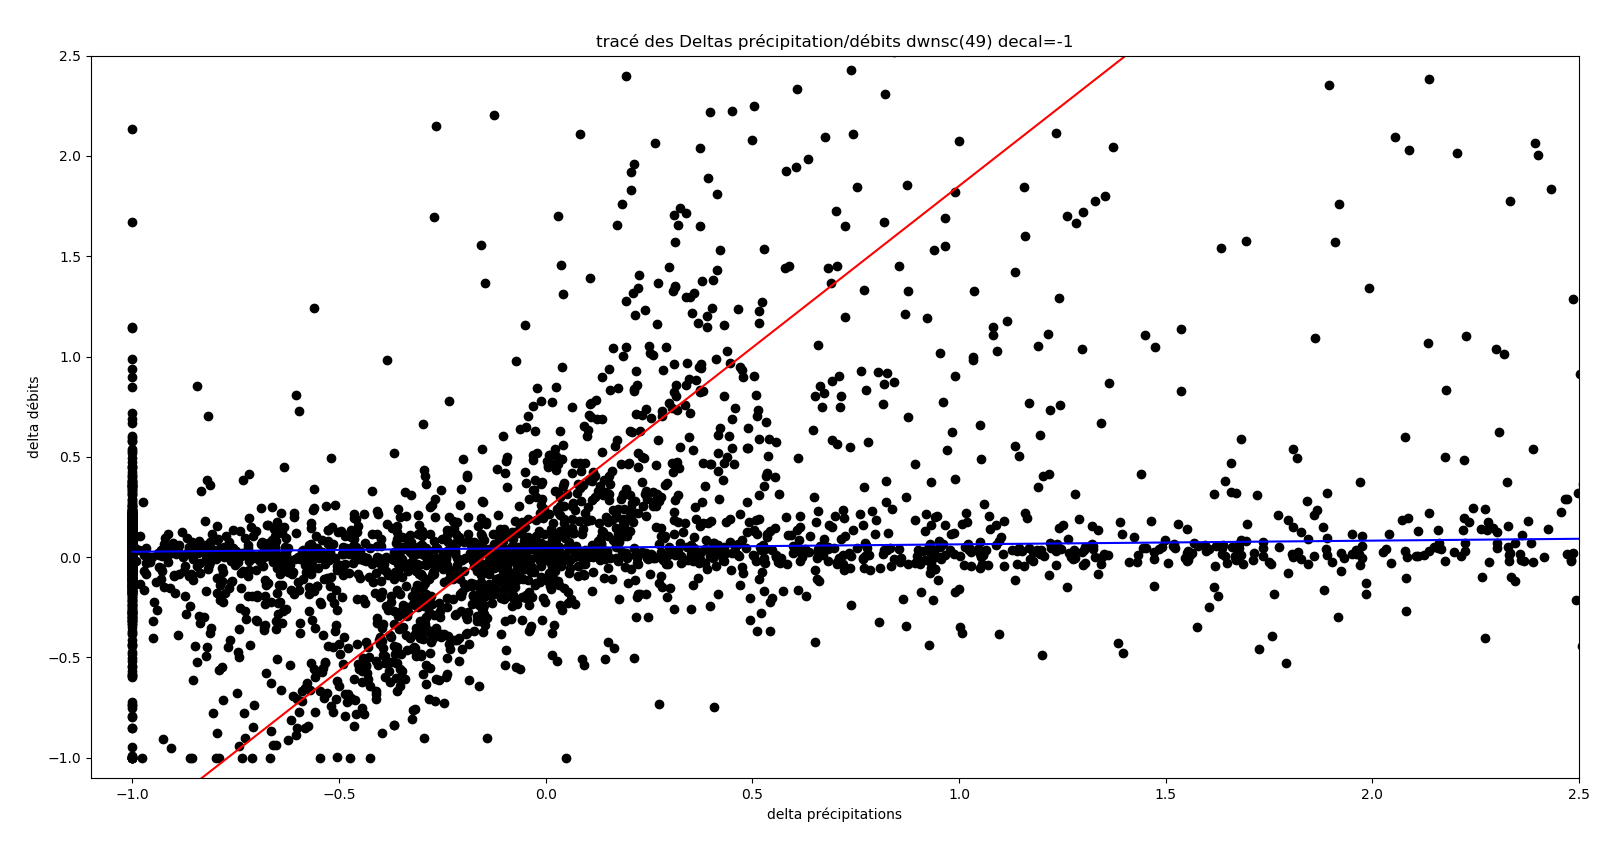
\includegraphics[scale=0.28]{images/deb_prec_dec1_droites.png}
		\captionof{figure}{tracé des $\Delta Q(t)$ en fonction des $\Delta R(t-1)$ avec droites de classification}
	\end{center}
	
	
	\newpage
	\bibliographystyle{apalike}
	\bibliography{mabib}
	
\end{document}